%Dokumentklasse
\documentclass[a4paper,12pt,twoside]{scrreprt}
\usepackage[left = 2.5cm, right = 2.5cm, top = 2.5 cm, bottom = 2.5cm]{geometry}
\linespread{1}


% Dokumentinformationen
\usepackage[
	pdftitle={Hamiltonian Systems with Constraints},
	pdfsubject={},
	pdfauthor={Eugen Dizer},
	pdfkeywords={}
	pdftex=true, 
	colorlinks=true,
 	breaklinks=true,
	citecolor=black,
	linkcolor=black,	
	menucolor=black,	
	urlcolor=black
]{hyperref}



% Standard Packages
\usepackage[utf8]{inputenc}
\usepackage[english]{babel}
\usepackage{graphicx}
\usepackage{graphicx, subfigure}
\graphicspath{{img/}}
\usepackage{lmodern}
\usepackage{color}
\usepackage{multicol}
\usepackage{transparent}
\usepackage{tabularx}
\usepackage{varioref}
\usepackage{hyperref}
\usepackage{setspace}
\usepackage{wrapfig}
\usepackage{caption}
\usepackage{textcomp}
\usepackage{enumitem}
\usepackage{pdfpages}
\usepackage{float}
\usepackage{fancyhdr}
% zusätzliche Schriftzeichen der American Mathematical Society
\usepackage{amsfonts}
\usepackage{amsmath,bm}
\usepackage{amssymb}
\usepackage{amsthm}
\usepackage{mathrsfs}


% nicht einrücken nach Absatz
\setlength{\parindent}{0pt}


% ============= Kopf- und Fußzeile =============

\pagestyle{fancy}

\fancyhf{}
\fancyhead[LE,RO]{\thepage}% gerade Seiten, links
\fancyhead[RE]{\slshape \leftmark}% gerade Seiten, rechts
\fancyhead[LO]{\slshape \rightmark}% ungerade Seiten, links

% ============= Package Einstellungen & Sonstiges ============= 

%Besondere Trennungen
%\hyphenation{De-zi-mal-tren-nung St-rei-fen-licht-scan-nern}
%\hyphenation{unserem}
%\hyphenation{ersten}

\newtheorem{definition}{Definition}
\newtheorem{theorem}{Theorem}
\newtheorem{exercise}{Exercise}
\newtheorem{example}{Example}

\newenvironment{solution}
               {\begin{proof}[\bfseries\upshape Solution\nopunct:]
               \renewcommand{\qedsymbol}{}
               \end{proof}}
               
\usepackage{xpatch}
\makeatletter
\xpatchcmd{\@thm}{\thm@headpunct{.}}{\thm@headpunct{}}{}{}
\makeatother

\addto{\captionsenglish}{\renewcommand{\bibname}{Literature}}

% ============= Dokumentbeginn =============

\begin{document}

\pagestyle{empty}
\begin{center}
\begin{tabular}{p{\textwidth}}

\vspace*{1cm}


\begin{center}
\linespread{1.2}
\LARGE{\textbf{Lecture Notes on \\
Hamiltonian Systems with Constraints\\
}}
\end{center}


\vspace*{0.5cm}

\begin{center}
given by
\end{center}


\begin{center}
\linespread{2}
Prof. Vladimir V. Vechernin \\
High Energy and Elementary Particle Physics \\ 
Saint Petersburg State University \\ 
Saint Petersburg, Russia \\
Winter Term 2018/19
\end{center}


\vspace*{1cm}


\begin{center}

\includegraphics[scale=0.1]{img/uni}
\end{center}



\vspace*{2cm}

\begin{center}
Typesetted by Eugen Dizer, \url{eugen9898@web.de}
\end{center}


\end{tabular}
\end{center}

\newpage
%Seitennummerierung neu beginnen, Zahlen [arabic], röm.Zahlen [roman,Roman], Buchstaben [alph,Alph]
\pagenumbering{roman}

\renewcommand{\chapterheadstartvskip}{\vspace{0pt}}
\renewcommand{\chapterheadendvskip}{\vspace{10pt}}

\setkomafont{section}{\Large}
\setkomafont{chapter}{\LARGE}

\addcontentsline{toc}{chapter}{Preface}
\chapter*{Preface}

These are the lecture notes on "Hamiltonian Systems with Constraints" given by Prof. Vechernin at Saint Petersburg State University which I typesetted in \LaTeX \ during my exchange semester in the winter term 2018/19. \\

The main reason for doing this was to enable the Russian students a better preparation for the exam because such typesetted notes didn't exist. Moreover, such a lecture wasn't offered at my home university which is the reason why I wanted to share the material with all students, who are curious about it, and translate the notes from Russian into English. Last but not least, the content is very interesting, in my opinion, and it is nice to have a small memory of the great time in Saint Petersburg. \\

The course is aimed for third-year undergraduate physics students who already have knowledge in classical mechanics, electrodynamics and quantum mechanics. One should be especially familiar with tensors and index notation, e.g. the Lagrangian description of electrodynamics is assumed to be known.
We will concentrate on the Hamiltonian method and the consequences of constraints. Some aspects might be missed, so there is no entitlement to completeness and this notes should be understood more like an introduction. \\

The first chapter contains some theory which is needed to analyse constrainted systems. In the following chapters, we use the knowledge to investigate some interesting examples and develop the theory further.
Sometimes, I changed the notation or the order to make it more readable and clear but I wanted to be as near to the lecture as possible to conserve the Russian style. In the end, there is a set of exercises for preparation for the exam.  \\

The lecture is based on the literature on the next page. Dirac was the first who realized the importance of this topic and developed the theory, so especially \cite{1} should be consultated for further reading and better explanations. \\

I would like to thank Ksusha for her beautiful and detailed handwritten notes and her help during the semester. \\


If you find any mistakes, please let me know. \\


January 03, 2019 \hfill Eugen Dizer 

\newpage
\addcontentsline{toc}{chapter}{Literature} 
\nocite*
\bibliographystyle{plaindin}
\bibliography{Literatur}


\newpage
\addtocontents{toc}{\protect\thispagestyle{empty}}
\tableofcontents


\newpage
\pagenumbering{arabic}
\pagestyle{fancy}
\chapter{Introduction}

The constraints, that we are talking about here, are not like the constraints in classical mechanics. They appear when we try to get from the Lagrange to the Hamilton formalism. 
\begin{itemize}
\item $L(q_i,\dot{q}_i)$, \ where $i = 1, ..., n$ degrees of freedom \\
The mechanical properties of a system are completly described by the Lagrangian. 
\end{itemize}
We will study constraints from a mathematical point of view, not a physical:
\begin{itemize}
\item Classical mechanics: physical constraints lead to changes in the mathematical description.
\item Now: most general description of Hamiltonian theory. The constraints will follow from the Lagrangian.
\end{itemize}

Why do we need the Hamilton formalism? \\
The most important fact is that a Hamiltonian system (described by coordinates $q_i$ and momenta $p_i$) can be quantized in a canonical way:
\begin{align}
L(q_i,\dot{q}_i) \ \longrightarrow \ H(q_i,p_i) \ \longrightarrow \ H(\hat{q}_i,\hat{p}_i) .
\end{align}
Nowadays, there are of course other methods of quantization, like the Feynman path integral, but we won't focus on quantization here. For us, it is important to know what happens when we try to get from the Lagrangian to the Hamiltonian. \\

How does it work?
\begin{enumerate}
\item Calculate the generalized momenta
\begin{align}\label{eq:momentum}
q_i \ \longrightarrow \ p_i \equiv \frac{\partial L(q_i,\dot{q}_i)}{\partial \dot{q}_i}.
\end{align}
This step is always possible, it results in $p_i(q_i,\dot{q}_i)$.
\item Build the Hamiltonian
\begin{align}\label{eq:hamilton}
H(q_i,p_i) = \sum_{i = 1}^n p_i \dot{q}_i - L(q_i,\dot{q}_i).
\end{align}
The expression on the right side still contains the velocities $\dot{q}_i$, so we have to express them through the generalized coordinates and momenta, by inverting \eqref{eq:momentum}
\begin{align}
p_i(q_i,\dot{q}_i) \longrightarrow \dot{q}_i = \dot{q}_i(q_i,p_i),
\end{align}
and insert in the equation \eqref{eq:hamilton}. Sometimes (if the Lagrangian is degenerate), this step is not possible. We will investigate, what to do in this cases.
\end{enumerate} 

We will start with discrete and finite dimensional systems and then move on to continuous systems by introducing field theoretical aspects.
\chapter{The Hamiltonian Method}
\section{Basics}
\begin{definition}
If the determinant of the matrix 
\begin{align}
a_{ik} = \frac{\partial^2 L(q_m,\dot{q}_m)}{\partial \dot{q}_i \partial \dot{q}_k}
\end{align}
vanishes, the Lagrangian is called degenerate. Otherwise, $L$ is nondegenerate or regular.
\end{definition}
When the Lagrangian is degenerate, some of the velocities $\dot{q}_i$ can disappear when we try to find $p_i(q_i,\dot{q}_i)$. We are left with an equation depending on the coordinates and momenta, called a constraint.
\begin{definition}[Primary constraint]
Equations of the form
\begin{align}
\phi_m(q_i,p_i) = 0, 
\end{align}
where $m = 1, ..., M$ is the number of constraints, are called primary constraints when they follow from the definition of the generalized momentum.
\end{definition}
Let's illustrate what these constraints mean. One can visualize the state of a mechanical system with $n$ degrees of freedom as a point $(q_i,p_i)$ in a $2n$-dimensional phase space ($n$ coordinates and $n$ momenta). The coordinates of this point (the state) depend on time and evolve according to the Hamiltonian equations of motion. 
\begin{figure}[H]
\begin{center}
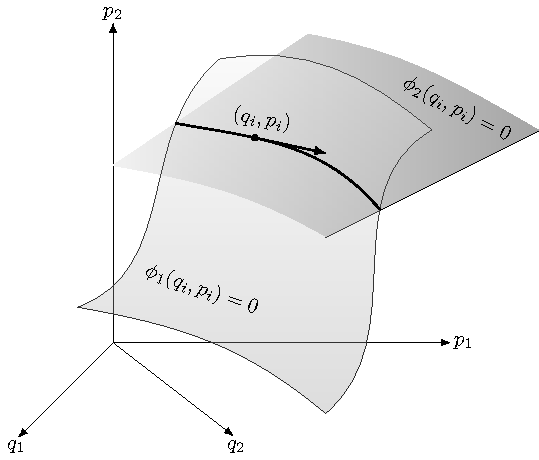
\includegraphics[scale=1.28]{img/constraint.pdf}
\end{center}
\caption{Two intersecting constraint surfaces. The system is only allowed to be in states in which both constraints are fulfilled.}
\label{fig:1}
\end{figure}
In general, the trajectory of this point can fill the whole phase space. When we have constraints, the system is only allowed to be in states in which the constraints are fulfilled. In phase space, they build hypersurfaces on which the point is allowed to move. If every constraint can be fulfilled, the point will move on the intersections of all constraints, like visualized in Fig. \ref{fig:1}. But how to include this into the mathematical formalism? \\
To see, how the constraints enter into the Hamiltonian equations of motion
\begin{align}
\dot{q}_i &= \frac{\partial H}{\partial p_i} \label{eq:1} \\
\dot{p}_i &= - \frac{\partial H}{\partial q_i} \label{eq:2}
\end{align}
and change the dynamics, it will be very useful to write them with Poisson brackets.
\begin{definition}[Poisson bracket]
\begin{align}
\left \{ f(q_i, p_i),g(q_i, p_i) \right \} \equiv \sum_{i=1}^n \left( \frac{\partial f}{\partial q_i} \frac{\partial g}{\partial p_i} - \frac{\partial g}{\partial q_i} \frac{\partial f}{\partial p_i} \right).
\end{align}
\end{definition}
Some properties of the Poisson bracket are:
\begin{enumerate}
\item \(
\begin{aligned}[t]
\left \{ f,g \right \} = - \left \{ g,f \right \}
\end{aligned} \) \ - \ anticommutative
\item \(
\begin{aligned}[t]
\left \{ \alpha f_1 + \beta f_2,g \right \} = \alpha \left \{ f_1,g \right \} + \beta \left \{ f_2,g \right \} 
\end{aligned} \) \ - \ bilinear
\item \(
\begin{aligned}[t]
\left \{  f_1 f_2,g \right \} = f_1 \left \{ f_2,g \right \} + f_2 \left \{ f_1,g \right \} 
\end{aligned} \) \ - \ "derivative"
\item \(
\begin{aligned}[t]
\left \{ \left \{ f,g \right \},h \right \} + \left \{ \left \{ g,h \right \},f \right \} + \left \{ \left \{ h,f \right \},g \right \} = 0 
\end{aligned} \) \ - \ Jacobi identity
\end{enumerate}
These rules hold for any three functions $f,g,h$ of phase space and time (observables).
\begin{theorem}\label{theorem}
The time evolution for any observable $g(q_i,p_i)$ is
\begin{equation}\label{eq:3}
\dot{g} = \frac{dg}{dt} = \left \{ g,H \right \}. 
\end{equation}
It is equivalent to the Hamiltonian equations of motion.
\end{theorem}
\begin{proof}
"$\Rightarrow$" By definition of the total derivative we have
\begin{align}
\frac{dg}{dt} = \sum_{i=1}^n \left( \frac{\partial g}{\partial q_i} \dot{q}_i + \frac{\partial g}{\partial p_i} \dot{p}_i \right) = \sum_{i=1}^n \left( \frac{\partial g}{\partial q_i} \frac{\partial H}{\partial p_i} - \frac{\partial g}{\partial p_i} \frac{\partial H}{\partial q_i} \right) = \left \{ g,H \right \},
\end{align}
where we used the Hamiltonian equations of motion \eqref{eq:1} and \eqref{eq:2}. \\
"$\Leftarrow$" Choose $g = q_k$ and get
\begin{align}
\dot{q}_k = \left \{ q_k,H \right \} = \frac{\partial H}{\partial p_k}.
\end{align}
Analog, with $g = p_k$ we get
\begin{align}
\dot{p}_k = \left \{ p_k,H \right \} = - \frac{\partial H}{\partial q_k}.
\end{align}
\end{proof}
From now on, we will use equation \eqref{eq:3} when we talk about equation of motion. This notation has the big advantage that it can be generalized directly under quantization:
\begin{align}
\left \{ f,g \right \} \  \longrightarrow \ \frac{1}{i \hbar} \ [\hat{f},\hat{g}].
\end{align}
So when we quantize our system and $\hat{g}(\hat{q}_i,\hat{p}_i)$ is an operator, the equation of motion take the form
\begin{align}
\frac{d}{dt}\hat{g} = \frac{i}{\hbar} \ [\hat{H} , \hat{g}],
\end{align}
which is equivalent to the Heisenberg and Schrödinger equation.


\section{From the Lagrangian to the Hamiltonian}
Suppose we have a Lagrangian $L = L(q_i,\dot{q}_i)$. The first step to get the Hamiltonian
\begin{align}
q_i \longrightarrow p_i \equiv \frac{\partial L(q_i,\dot{q}_i)}{\partial \dot{q}_i} = p_i(q_i,\dot{q}_i)
\end{align}
is always possible because one can still differentiate, even when $L$ is degenerate.
For the next step, to express the Hamiltonian only through $q_i$ and $p_i$, it can happen that some velocities $\dot{q}_k$ vanish when we try to calculate the generalized momenta. In this case, it is not possible to express $\dot{q}_k$ through the conjugated momentum $p_k$ and we are left with a primary constraint. So we have not set them by hand, they arised from the definition of the generalized momentum. But there is a nice theorem:
\begin{theorem}
Even if we cannot invert the definition of the generalized momentum and express some velocities through their momenta, 
\begin{align}
H(q_i,\dot{q}_i) = \sum_{i=1}^{n} \dot{q}_i p_i(q_i,\dot{q}_i) - L(q_i,\dot{q}_i), 
\end{align}
is still a function of the coordinates and momenta, all velocities can be eliminated.
\end{theorem}
\begin{proof}
The variation of this function is
\begin{align}
\delta H(q_i,\dot{q}_i) &= \sum_{k=1}^{n} \left( \frac{\partial H}{\partial q_k} \delta q_k + \frac{\partial H}{\partial \dot{q}_k} \delta \dot{q}_k \right) \notag \\
&= \sum_{k=1}^{n} \left( \sum_{i=1}^n \dot{q}_i \frac{\partial p_i}{\partial q_k} - \frac{\partial L}{\partial q_k} \right) \delta q_k + \sum_{k=1}^n \left( p_k + \sum_{i=1}^n \dot{q}_i \frac{\partial p_i}{\partial \dot{q}_k} - \frac{\partial L}{\partial \dot{q}_k} \right) \delta \dot{q}_k \notag \\
&= \sum_{i=1}^{n} \dot{q}_i \left( \sum_{k=1}^n \frac{\partial p_i}{\partial q_k} \delta q_k + \sum_{k=1}^n \frac{\partial p_i}{\partial \dot{q}_k} \delta \dot{q}_k \right) - \sum_{k=1}^n \frac{\partial L}{\partial q_k} \delta q_k \notag \\
&= \sum_{i=1}^n \dot{q}_i \delta p_i - \sum_{i=1}^n \frac{\partial L}{\partial q_i} \delta q_i.
\end{align}
Since we can rewrite the variation in terms of $\delta q_i$ and $\delta p_i$, the Hamiltonian can be expressed as a function of the coordinates and momenta only.
\end{proof}
Comparing the terms in the last line with the variation of $H$ with respect to $\delta q_i$ and $\delta p_i$ and using the Euler-Lagrange-equation, one can find the Hamilton equations of motion. \\
But it is not so easy after all. Remember that we still can have primary constraints $\phi_m$ with vanashing variation:
\begin{align}
\delta \phi_m = 0 = \sum_{i=1}^n \left( \frac{\partial \phi_m}{\partial q_i} \delta q_i + \frac{\partial \phi_m}{\partial p_i} \delta p_i \right).
\end{align}
So we could add this variation to the variation of the Hamiltonian without changing it. This is very useful because normally, $M$ constraints would result in $2n - M$ independent equations of motion but most times, it is easier just to add $M$ independent arbitrary coefficients/functions than reducing the number of equations. So we return the lost degrees of freedom by multiplying our constraints with arbitrary functions $u_m$ and adding them to our variation.
Continuing this idea, since the variation of the constraints is zero, we can add
\begin{align}
0 = \sum_{m=1}^M u_m \delta \phi_m = \sum_{m=1}^M u_m \sum_{i=1}^n \left( \frac{\partial \phi_m}{\partial q_i} \delta q_i + \frac{\partial \phi_m}{\partial p_i} \delta p_i \right)
\end{align}
to 
\begin{align}
\sum_{i=1}^n \left( \frac{\partial H}{\partial p_i} - \dot{q}_i \right) \delta p_i + \sum_{i=1}^n \left( \frac{\partial H}{\partial q_i} + \dot{p}_i \right) \delta q_i = 0,
\end{align}
where we used the Hamilton equations of motion, and get
\begin{align}
\frac{\partial H}{\partial p_i} + \sum_{m=1}^M u_m \frac{\partial \phi_m}{\partial p_i} &= \dot{q}_i \\
\frac{\partial H}{\partial q_i} + \sum_{m=1}^M u_m \frac{\partial \phi_m}{\partial q_i} &= - \dot{p}_i,
\end{align}
which are $2n$ equations with $M$ independent extra-functions. 
It looks like these extra-functions were added to the Hamiltonian, so the following definition is reasonable:
\begin{definition}[Total Hamiltonian]
\begin{align}
H_T(q_i,p_i) \equiv H(q_i,p_i) + \sum_{m=1}^M u_m(q_i,p_i) \phi_m(q_i,p_i).
\end{align}
\end{definition}
Now we want to adapt our results to the formulations of the equations of motion with Poisson brackets. We claim that
\begin{align}
\dot{g} = \left \{ g,H_T \right \} &= \left \{ g,H \right \} + \sum_{m=1}^M u_m  \left \{ g,\phi_m \right \} + \sum_{m=1}^M \left \{ g,u_m \right \} \phi_m \notag \\
&\approx \left \{ g,H \right \} + \sum_{m=1}^M u_m  \left \{ g,\phi_m \right \},
\end{align}
where we have used that all constraints are zero on the constraint surface in the last step. The proof is analog to the proof of Theorem~\ref{theorem}. \\

At this point, we should say something about the usage of constraints and \textit{weak equalities}. First of all, we are not allowed to use the constraints inside a Poisson bracket. We have to calculate the Poisson bracket first and then apply the constraint when it is outside the bracket. If two quantities $f,g$ differ only by a linear combination of constraints, we call them weakly equal (denoted by $f \approx g$). We will use this notation sometimes to distinguish them from usual or strong equations.

\begin{example}
Consider the Lagrangian
\begin{align}
L = L(q,\dot{q}) = q \dot{q} - \frac{q^2}{2}.
\end{align}
From the definition of the generalized momentum follows a primary constraint:
\begin{align}
p = \frac{\partial L}{\partial \dot{q}} = q \ \ \ \Longrightarrow \ \ \ \phi_1 = p - q = 0.
\end{align}
Because of this constraint, the Hamiltonian is not unique:
\begin{align}
H = \dot{q} p - L = \frac{q^2}{2} = \frac{p^2}{2} = \frac{q p}{2}.
\end{align}
This arbitrariness is included in the total Hamiltonian:
\begin{align}
H_T = \frac{q^2}{2} - u_1(q,p) (p-q).
\end{align}
Depending on the choice of $u_1(q,p)$, we can switch from one form to another.
\end{example}

Realizing the appearance of unknown functions in the Hamiltonian and the equations of motion, one might develop bad thoughts about determinism and the predictability of the future.
It turns out that everything keeps predictable and the unknown functions aren't a big problem after all. We will see later that they correspond to mathematical degrees of freedom, so called gauge transformations. \\

For now, let us focus on the consistency of our theory. When we choose the initial conditions, we have to assure ourself that they fulfill the constraints. After time, the equations of motion could lead to a point in phase space which is not on the constraint surface. How to ensure that the system doesn't leave the constraint surface?
Since we want that the primary constraints are fulfilled at every moment, we require
\begin{align}\label{eq:4}
0 \overset{!}{=} \dot{\phi}_k = \left \{ \phi_k,H \right \} + \sum_{m=1}^M u_m  \left \{ \phi_k,\phi_m \right \},
\end{align}
for $k=1,...,M$. This can lead to four cases. First, it could lead directly to an inconsistency saying that the Lagrangian describes no proper system. Second, it could be satisfied identically and we can be sure that everything will be fine. Third, it can lead to an equation that determines the unknown functions and reduces the degrees of gauge freedom. Fourth, it can lead to other constraints, called \textit{secondary constraints}:
\begin{align}\label{eq:5}
0 = \dot{\phi}_1 = \left \{ \phi_1,H \right \} + \sum_{m=1}^M u_m  \left \{ \phi_1,\phi_m \right \} = \left \{ \phi_1,H \right \} = \chi(q,p).
\end{align}
They differ from the primary constraints in the fact that the primary constraints are merely a consequence of the definition of the generalized momenta, while for the secondary constraints, one has to make use of the Lagrangian equations of motion as well. \\
If we have a secondary constraint, then we get another consistency condition because we can work out again $\dot{\chi}$ according to the equation of motion and require that $\dot{\chi} = 0$. This equation has to be treated on the same footing as \eqref{eq:4}. One must again see to which case it leads. If it leads to another secondary constraint, we have to push the process one stage further and check the consistency condition again. \\
We carry on like that until we have exhausted all the consistency conditions, and the final result will be that we are left with a number of secondary constraints together with a number of conditions on the functions $u_m$. The process \footnote{It should be mentioned that it is a controversial topic whether every new constraint should be added to the total Hamiltonian with an undetermined function after each step or not. It only makes a difference when we generate second-class constraints during our procedure. For the most cases, Dirac's procedure (without adding the secondary constraints to the Hamiltonian) works out and leads to the right physics. If one has second-class constraints, one should pay attention and ponder what to do. There are even examples where adding secondary constraints to the Hamiltonian leads to wrong results. That's why we will stick to Dirac and describe his method.} is described in detail by Dirac in his lectures on quantum mechanics \cite{1}. \\

Let's take a closer look on the secondary constraints now. Since they are treated for many purposes like primary constraints, we will denote them like
\begin{align}
\phi_{M+1}(q_i,p_i), ... , \phi_J(q_i,p_i)
\end{align}
and require now 
\begin{align}\label{eq:6}
\dot{\phi}_j = \left \{ \phi_j,H \right \} + \sum_{m=1}^M u_m  \left \{ \phi_j,\phi_m \right \} = 0, 
\end{align}
for $j=1,...,M,M+1,...,J$. These are a number of non-homogeneous linear equations for the unknown functions $u_m$. Let us investigate the solvability of this system. Suppose that we are at the beginning of our procedure and have no secondary constraints yet. Then we can introduce the matrix $\hat{a}$ with components
\begin{align}
a_{jm} = \left \{ \phi_j,\phi_m \right \}, \ \ j,m = 1, \dots, M.
\end{align}
With equation \eqref{eq:6} it follows that
\begin{align}
\sum_{m=1}^M a_{jm} u_m = b_j = - \left \{ \phi_j,H \right \},
\end{align}
which expresses the linear equation system in matrix form. Since the rank of this matrix can be between 0 and $M$:
\begin{align}
0 \leq \text{rank} (\hat{a}) \leq M,
\end{align}
there are two options for solutions of this system. 

\pagebreak

\begin{enumerate}
\item If the rank of the $M \times M$ matrix is maximal, then one has a minimal system of $M$ equations with $M$ variables.
There exists a unique solution 
\begin{align}
u_m = U_m(q_i,p_i).
\end{align}
\item If the rank of the $M \times M$ matrix is $\leq M-1$, then there exist eigenvectors
\begin{align}\label{eq:7}
u_m = U_m(q_i,p_i) + \sum_{a=1}^A v_a(q_i,p_i) V_m^{(a)}(q_i,p_i),
\end{align}
where $A = M - \text{rank} (\hat{a})$ with arbitrary coefficients $v_a$ and any solution $V_m^{(a)}(q_i,p_i)$ of the homogeneous equations. They satisfy 
\begin{align}
\sum_{m=1}^M a_{jm} U_m = b_j \ \ \ \text{and} \ \ \ \sum_{m=1}^M a_{jm} V_m^{(a)} = 0.
\end{align}
The solution is not unique.
\end{enumerate}

Inserting \eqref{eq:7} in the total Hamiltonian, we get
\begin{align}\label{eq:8}
H_T(q_i,p_i) &= H + \sum_{m=1}^M U_m \phi_m + \sum_{a=1}^A v_a \left( \sum_{m=1}^M V_m^{(a)} \phi_m \right) \notag \\
&= H' + \sum_{a=1}^A v_a \tilde{\phi}_a.
\end{align}
Depending on how much the rank of the matrix $\hat{a}$ is smaller than $M$, we are left with $A = M - \text{rank} (\hat{a})$ constraints. So after the procedure, we can find some unknown functions $u_m$ and reduce their degree of freedom in some cases. The general rules are:
\begin{enumerate}
\item If the $u$'s vanish $\longrightarrow$ introduce secondary constraints
\item If not $\longrightarrow$ find conditions on the $u$'s and reduce their degree of freedom.
\end{enumerate}


For the following analysis, we introduce a useful terminology:
\begin{definition}[First-class quantity]
A quantity $R(q_i,p_i)$ is first-class, if it has zero Poisson brackets with all the $\phi$'s:
\begin{align}
\left \{ R,\phi_j \right \} = \sum_{j' = 1}^J r_{j j'} \phi_{j'} \approx 0,
\end{align}
where $j = 1, ... , J$. Otherwise, $R$ is second-class.
\end{definition}
It is important to find all constraints first and then talk about what is first-class and second-class. The following theorem shows a nice property of first-class quantities.

\pagebreak

\begin{theorem}
The Poisson bracket of two first-class quantities is also first-class.
\end{theorem}
\begin{proof}
Let $R,S$ be first-class. Then we have 
\begin{align}
\left \{ R,\phi_j \right \} &= \sum_{j' = 1}^J r_{j j'} \phi_{j'} \approx 0 \\
\left \{ S,\phi_j \right \} &= \sum_{j' = 1}^J s_{j j'} \phi_{j'} \approx 0.
\end{align}
Using the Jacobi identity and the Einstein summation convention, we have
\begin{align}
\left \{ \left \{ R,S \right \},\phi_j \right \} &= \left \{ \left \{ R,\phi_j \right \},S \right \} - \left \{ \left \{ S,\phi_j \right \},R \right \} \notag \\
&= \left \{ r_{j j'} \phi_{j'},S \right \} - \left \{ s_{j j'} \phi_{j'},R \right \} \notag \\
&= r_{j j'} \left \{ \phi_{j'},S \right \} + \left \{ r_{j j'},S \right \} \phi_{j'} - s_{j j'} \left \{ \phi_{j'},R \right \} - \left \{ s_{j j'},R \right \} \phi_{j'} \notag \\
&\approx 0.
\end{align}
\end{proof}

It turns out that our Hamiltonian in equation \eqref{eq:8} is first-class. To see this, check that every term is first-class:
\begin{itemize}
\item \(
\begin{aligned}[t]
\left \{ H',\phi_j \right \} &= \left \{ H + \sum_{m=1}^M U_m \phi_m ,\phi_j \right \} \approx  \left \{ H ,\phi_j \right \} + \sum_{m=1}^M U_m \left \{ \phi_m ,\phi_j \right \} \notag \\
&= b_j - \sum_{m=1}^M a_{jm} U_m = b_j - b_j = 0.
\end{aligned} \)
\item \(
\begin{aligned}[t]
\left \{ v_a \tilde{\phi}_a,\phi_j \right \} \approx v_a \left \{\tilde{\phi}_a,\phi_j \right \} = v_a \sum_{m=1}^M V_m^{(a)} \left \{ \phi_m ,\phi_j \right \} = - v_a \sum_{m=1}^M a_{jm} V_m^{(a)} = 0.
\end{aligned} \)
\end{itemize}


\section{Examples}

Now, we present two typical exersices. Consider the Lagrangian
\begin{align}
L = \frac{1}{2} \left[ \left( \frac{d}{dt} - y \right) x \right]^2 = \frac{1}{2} \left(\dot{x} - xy \right)^2.
\end{align}
First, calculate the conjugate momentum:
\begin{align}
p_x &= \frac{\partial L}{\partial \dot{x}} = \dot{x} - xy \\
p_y &= \frac{\partial L}{\partial \dot{y}} = 0.
\end{align}
From here, we get our first constraint: $\phi_1 = p_y = 0$. \\

The Hamiltonian is given by
\begin{align}
H &= \dot{x} p_x + \dot{y} p_y - \frac{1}{2} \left(\dot{x} - xy \right)^2 \notag \\
&= (p_x + xy)p_x - \frac{1}{2} p_x^2 \notag \\
&= \frac{1}{2} p_x^2 + xy p_x.
\end{align}
But it is not unique. The full Hamiltonian is
\begin{align}
H_T = H + u(x,p_x,y,p_y) \phi_1.
\end{align}
In the following, we will write $u = u(x,p_x,y,p_y)$ but keep in mind that it depends on all these variables. We get the equation of motion by
\begin{align}
\dot{g} = \left \{ g,H \right \} + u \left \{ g,\phi_1 \right \}.
\end{align}
We notice that
\begin{align}
0 = \dot{\phi}_1 = \left \{ \phi_1,H \right \} + u \left \{ \phi_1,\phi_1 \right \} = \left \{ p_y,\frac{1}{2} p_x^2 + xy p_x \right \} = \left \{ p_y,y \right \} x p_x = - x p_x.
\end{align}
Which leads to a secondary constraint:
\begin{align}
\left.
\begin{array}{llll}
      \text{Either:} & x = 0 & \Rightarrow &  p_x = 0 \\
      \text{Or:} & p_x = 0
\end{array}
\right \} \Longrightarrow \phi_2 = p_x = 0.
\end{align}
Let's check whether it satisfies the condition that we required for a constraint: 
\begin{align}
0 \overset{?}{=} \dot{\phi}_2 = \left \{ \phi_2,H \right \} + u \left \{ \phi_2,\phi_1 \right \} = \left \{ p_x,\frac{1}{2} p_x^2 + xy p_x \right \} = \left \{ p_x,x \right \} y p_x = - y p_x \approx 0.
\end{align}
So it is consistent and we get no more constraints. We can also check that $\phi_1, \phi_2$ and $H$ are first-class. We show it only for $H$:
\begin{align}
\left \{ H,\phi_1 \right \} &= \left \{ \frac{1}{2} p_x^2 + xyp_x, p_x \right \} = y p_x \approx 0 \\
\left \{ H,\phi_2 \right \} &= \left \{ \frac{1}{2} p_x^2 + xyp_x, p_y \right \} = x p_x \approx 0.
\end{align}


Another example which is quite similar to string theory, is the following. 
\begin{align}
L = q_1 q_2 (\dot{q}_1 + \dot{q}_2).
\end{align}
Following the procedure, we get two primary constraints:
\begin{align}
p_1 &= \frac{\partial L}{\partial \dot{q}_1} = q_1 q_2 \ \ \ \Longrightarrow \ \ \ \phi_1 = p_1 - q_1 q_2 = 0. \\
p_2 &= \frac{\partial L}{\partial \dot{q}_2} = q_1 q_2 \ \ \ \Longrightarrow \ \ \ \phi_2 = p_2 - q_1 q_2 = 0.
\end{align}
The Hamiltonian is
\begin{align}
H = \dot{q}_1 p_1 + \dot{q}_2 p_2 - q_1 q_2 (\dot{q}_1 + \dot{q}_2) = 0.
\end{align}
At this point, it is useful to notice the following theorem. \\

\begin{theorem}
\label{Theorem}
If the Lagrangian $L$ is homogeneous of degree $1$ in the velocities  
\begin{align}
L(q_i,\lambda \dot{q}_i) = \lambda L(q_i,\dot{q}_i), \label{eq:9}
\end{align}
then $H(q_i,p_i) = 0$.
\end{theorem}
\begin{proof}
The proof of this theorem is analog to the proof of Euler's homogeneous function theorem. 
Differentiating both sides of equation \eqref{eq:9} with respect to $\lambda$ yields
\begin{align}
L(q_i,\dot{q}_i) = \frac{\partial L(q_i,\lambda \dot{q}_i)}{\partial \lambda} = \sum_k \dot{q}_k \frac{\partial L(q_i,\lambda \dot{q}_i)}{\partial (\lambda \dot{q}_k)} .
\end{align}
By setting $\lambda = 1$, we obtain
\begin{align}
\sum_k \dot{q}_k \frac{\partial L(q_i,\dot{q}_i)}{\partial \dot{q}_k} - L(q_i,\dot{q}_i) = H(q_i,p_i) = 0.
\end{align}
\end{proof}

So we didn't even have to calculate the Hamiltonian because our Lagrangian is homogeneous of degree $1$. \\

The total Hamiltonian is
\begin{align}
H_T = 0 + u_1 \phi_1 + u_2 \phi_2
\end{align}
and the equation of motion is
\begin{align}
\dot{g} = u_1 \left \{ g, \phi_1 \right \} + u_2 \left \{ g, \phi_2 \right \}.
\end{align}

With the identity $\{ q_i, p_k \} = \delta_{ik}$, we get $\{ \phi_1 , \phi_2 \} = q_2 - q_1$ and obtain a new (secondary) constraints out of the requirement that
\begin{align}
0 \overset{!}{=} \dot{\phi}_1 &= u_1 \left \{ \phi_1, \phi_1 \right \} + u_2 \left \{ \phi_1, \phi_2 \right \} = u_2 (q_2 - q_1) \\
0 \overset{!}{=} \dot{\phi}_2 &= u_1 \left \{ \phi_2, \phi_1 \right \} + u_2 \left \{ \phi_2, \phi_2 \right \} = u_1 (q_1 - q_2).
\end{align}
\textit{First case $\phi_3 = q_1 - q_2 = 0$.} \\
We have to check that this constraint fulfills our requirement too:
\begin{align}
0 \overset{!}{=} \dot{\phi}_3 &= u_1 \left \{ \phi_3, \phi_1 \right \} + u_2 \left \{ \phi_3, \phi_2 \right \} = u_1 - u_2.
\end{align}
This is just an additional condition on the functions $u_1$ and $u_2$, saying that $u_1 = u_2 = v$. \\

The total Hamiltonian is therefore
\begin{equation}
H_T = v ( \phi_1 + \phi_2 ).
\end{equation}
Now, we want to see whether the Hamiltonian is first-class or second-class. But have we found already all constraints? There is a theorem saying that there is always an even number of second-class constraints, if one cannot combine all secondary constraints to get a new primary constraint. We will proof it later but for now, in our case, we only have one secondary constraint, so we have to find more constraints by combining the old ones:
\begin{align}
\tilde{\phi}_1 &= \phi_1 + \phi_2 = 0 \\
\tilde{\phi}_2 &= \phi_1 - \phi_2 = 0.
\end{align}
And now check which of them are first-class or second-class:
\begin{itemize}
\item \(
\begin{aligned}[t]
\left \{ \tilde{\phi}_1,\tilde{\phi}_2 \right \} = \left \{ p_1 + p_2 - 2 q_1 q_2, p_1 - p_2 \right \} = 2 (q_1 - q_2) = 0.
\end{aligned} \)
\item \(
\begin{aligned}[t]
\left \{ \tilde{\phi}_1,\phi_3 \right \} = \left \{ p_1 + p_2 - 2 q_1 q_2, q_1 - q_2 \right \} = -1 + 1 = 0.
\end{aligned} \)
\item \(
\begin{aligned}[t]
\left \{ \tilde{\phi}_2,\phi_3 \right \} = \left \{ p_1 - p_2, q_1 - q_2 \right \} = -2.
\end{aligned} \)
\end{itemize}
So $\tilde{\phi}_1$, and therefore our Hamiltonian, is first-class and $\tilde{\phi}_2,\phi_3$ are second-class like we expected. We notice:
\begin{definition}
True secondary constraints are secondary constraints which one cannot combine to first-class quantities.
\end{definition}

\textit{Second case $q_1 \neq q_2 \Longrightarrow u_1 = u_2 = 0$.} \\
And the total Hamiltonian is zero.



\section{Gauge Transformations}
In this section, we will see the meaning of the arbitrary coefficients in the total Hamiltonian \eqref{eq:8}.
With the equation of motion, one can express little changes in the function $g$:
\begin{align}\label{eq:10}
\frac{\Delta g}{\Delta t} = \dot{g} = \left \{ g,H' \right \} + \sum_{a=1}^A v_a \left \{ g,\tilde{\phi}_a \right \}.
\end{align}
Since the $v_a$ are arbitrary, there are many possible results for $\Delta g$. The situation is illustrated in Fig.~\ref{fig:2}.

\begin{figure}[H]
\begin{center}
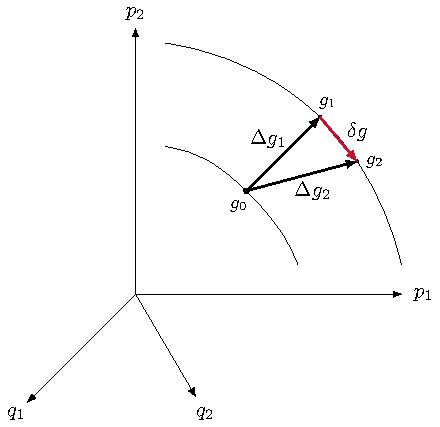
\includegraphics[scale=1.4]{img/gauge1.pdf}
\end{center}
\caption{Evolution of the observable $g$ in phase space.}
\label{fig:2}
\end{figure}

The time evolution of the observable $g$ for small intervals $\Delta t$ can be estimated as
\begin{align}
g(t + \Delta t) = g_0 + \Delta g,
\end{align}
where $\Delta g$ is given by equation \eqref{eq:10}:
\begin{align}
\Delta g = \left \{ g,H' \right \} \Delta t + \sum_{a=1}^A \left( v_a \Delta t \right) \left \{ g,\tilde{\phi}_a \right \}.
\end{align}

Let's choose two different $v_a^{(1)}$ and $v_a^{(2)}$ with which we land eather on $g_1$ or $g_2$, the corresponding change $\Delta g_i$ can be written as:
\begin{align}
\Delta g_1 &= \left \{ g,H' \right \} \Delta t + \sum_{a=1}^A \left( v_a^{(1)} \Delta t \right) \left \{ g,\tilde{\phi}_a \right \} \\
\Delta g_2 &= \left \{ g,H' \right \} \Delta t + \sum_{a=1}^A \left( v_a^{(2)} \Delta t \right) \left \{ g,\tilde{\phi}_a \right \}.
\end{align}

Different functions $v_a^{(i)}$ lead to different results $\Delta g_i$. This means that $g(t + \Delta t)$ is not well defined and depends on the functions $v_a^{(i)}$. The key to the solution of this problem is to say that all \textit{mathematical states} $g_i$ correspond to the same \textit{physical state} $g(t + \Delta t)$. Like in electrodynamics, where $\vec{A} \longrightarrow \vec{A}' = \vec{A} + \nabla f$ leaves the magnetic field unchanged. \\

The transformation which leads from $g_1$ to $g_2$ is called a \textit{gauge transformation}:
\begin{align}
g_1 \longrightarrow g_2 =  g_1 + \delta g.
\end{align}

Let us calculate the explicit form of $\delta g$:
\begin{align}
\delta g = \Delta g_2 - \Delta g_1 = \sum_{a=1}^A \left( v_a^{(2)} - v_a^{(1)} \right) \Delta t \left \{ g,\tilde{\phi}_a \right \} \equiv \sum_{a=1}^A \varepsilon_a \left \{ g,\tilde{\phi}_a \right \},
\end{align}
where $\varepsilon_a$ is a small, arbitrary parameter since $\Delta t$ is small.
\label{sec:gauge_transformations}
We see that this \textit{infinitesimal} change can be expressed as the Poisson bracket of $g$ with the primary constraints. We therefore say that primary constraints are generators of \textit{infinitesimal} gauge transforations. \\
More exactly, the first-class primary constraints are generators of gauge transformation since we started with a first-class total Hamiltonian. Later, we will learn more about the role of first-class quantities for gauge transformations. \\

Before continuing, we would like to illustrate gauge transformations with the following example.
Consider the Lagrangian
\begin{align}
L = \frac{1}{2} (x \dot{x} + y \dot{y})^2.
\end{align}
The definition of the generalized momentum 
\begin{align}
p_x &= \frac{\partial L}{\partial \dot{x}} =  x (x \dot{x} + y \dot{y}) \\
p_y &= \frac{\partial L}{\partial \dot{y}} = y (x \dot{x} + y \dot{y})
\end{align}
leads to the primary constraint
\begin{align}
\phi_1 = p_x y - p_y x = 0.
\end{align}
So again, the Hamiltonian is not unique:
\begin{align}
H &= \dot{x} p_x + \dot{y} p_y - \frac{1}{2} (x \dot{x} + y \dot{y})^2 \notag \\
&= x \dot{x} (x \dot{x} + y \dot{y}) + y \dot{y} (x \dot{x} + y \dot{y}) - \frac{1}{2} (x \dot{x} + y \dot{y})^2 \notag \\
&= (x \dot{x} + y \dot{y})^2 - \frac{1}{2} (x \dot{x} + y \dot{y})^2 \notag \\
&= \frac{1}{2} (x \dot{x} + y \dot{y})^2  \notag \\
&= \frac{p_x^2}{2 x^2} = \frac{p_y^2}{2 y^2} = \frac{p_x p_y}{2 x y}.
\end{align}
We therefore build the total Hamiltonian
\begin{align}
H_T = \frac{p_x^2}{2 x^2} + u_1 (p_x y - p_y x),
\end{align}
where the arbitrariness lies completely in the function $u_1$ now. By choosing $u_1$, one can change between the different variants. The equation of motion is given by
\begin{align}
\dot{g} = \left \{ g,H \right \} + u_1 \left \{ g,\phi_1 \right \}.
\end{align}
Let's check whether the consistency condition holds:
\begin{align}
0 = \dot{\phi}_1 &= \left \{ \phi_1,H \right \} + u_1 \left \{ \phi_1,\phi_1 \right \} = \left \{ p_x y - p_y x,\frac{p_x^2}{2 x^2} \right \} \notag \\
&= \frac{p_x^2 y}{2} \left \{ p_x,\frac{1}{x^2} \right \} - \frac{p_y}{2 x^2} \left \{ x,p_x^2 \right \} \notag \\
&= \frac{p_x^2 y}{2} \left(-(-2) \frac{1}{x^3}\right) - \frac{p_y}{2 x^2} 2 p_x \notag \\
&= \frac{p_x (p_x y - p_y x)}{x^3} \notag \\
&= \frac{p_x \phi_1}{x^3} \approx 0. \ \ \ \surd
\end{align}
So $u_1$ remains arbitrary and we have no secondary constraints. It follows that $\phi_1 = \phi$ is first-class (which is always the case when we only have one constraint) and act as a generator of gauge transformations:
\begin{align}
\Delta g = \varepsilon \left \{ g,\phi \right \}.
\end{align}
Let us insert $\phi$ and see which transformations don't change the physical state of the observables:
\begin{itemize}
\item $\Delta x = \varepsilon \left \{ x,\phi \right \} = \varepsilon \left \{ x,p_x y - p_y x \right \}= \varepsilon y$
\item $\Delta y = \varepsilon \left \{ y,\phi \right \} = - \varepsilon x$
\item $\Delta p_x = \varepsilon \left \{ p_x,\phi \right \} = \varepsilon p_y$
\item $\Delta p_y = \varepsilon \left \{ p_y,\phi \right \} = - \varepsilon p_x$.
\end{itemize}
These transformations do look like the infinitesimal version of rotations in $2$ dimensional space. So let us work out the connection. We will show it for the space part and the momentum is completely analogous.
The equations 
\begin{align}
x' &= x + \varepsilon y \\
y' &= y - \varepsilon x
\end{align}
can be written in matrix form like 
\begin{align}
\bar{r} \ ' = \bar{r} + \varepsilon \hat{\omega} \bar{r},
\end{align}
where
\begin{align}
\bar{r} = 
\begin{pmatrix}
    x \\
    y
\end{pmatrix} \ \ \ \text{and} \ \ \
\hat{\omega} = 
\begin{pmatrix}
    0 & 1 \\
    -1 & 0
\end{pmatrix}.
\end{align}
It follows that
\begin{align}
\Delta \bar{r} = \varepsilon \hat{\omega} \bar{r}.
\end{align}
Redefine the small parameter $\varepsilon \longrightarrow \Delta \alpha$ and solve the differential equation:
\begin{align}
\frac{\Delta \bar{r}}{\Delta \alpha} = \hat{\omega} \bar{r} \ \ \Longrightarrow \ \ \bar{r}(\alpha) = \exp(\hat{\omega} \alpha) \bar{r}(0).
\end{align}
To get a better feeling for what this means, we expand the solution into the Taylor series and note that
\begin{align}
\hat{\omega} = 
\begin{pmatrix}
    0 & 1 \\
    -1 & 0
\end{pmatrix}, \ \
\hat{\omega}^2 = - I, \ \
\hat{\omega}^3 = - \hat{\omega}, \ \
\hat{\omega}^4 = I, \ \
\hat{\omega}^5 = \hat{\omega}, \ \dots .
\end{align}
So 
\begin{align}
\bar{r}(\alpha) &= \left( I + \alpha \hat{\omega} + \frac{\alpha^2 \hat{\omega}^2}{2} + \frac{\alpha^3 \hat{\omega}^3}{3 !} + \frac{\alpha^4 \hat{\omega}^4}{4 !} + \dots  \right) \bar{r}(0) \notag \\
&= \Bigg [  \Big ( \underbrace{1 - \frac{\alpha^2}{2} + \frac{\alpha^4}{4 !} - \dots}_{\Large = \ \cos \alpha} \Big ) I + \Big ( \underbrace{\alpha - \frac{\alpha^3}{3 !} + \frac{\alpha^5}{5 !} - \dots}_{\Large = \ \sin \alpha} \Big ) \hat{\omega} \Bigg ] \bar{r}(0) .
\end{align}
\begin{align}
\Longrightarrow \ 
\begin{pmatrix}
    x' \\
    y'
\end{pmatrix} =
\begin{pmatrix}
    \cos \alpha & \sin \alpha \\
    - \sin \alpha & \cos \alpha
\end{pmatrix}
\begin{pmatrix}
    x \\
    y
\end{pmatrix}.
\end{align}
So our suggestion was right, the gauge transformations are really rotations.
We can illustrate this as follows:
\begin{figure}[H]
\begin{center}
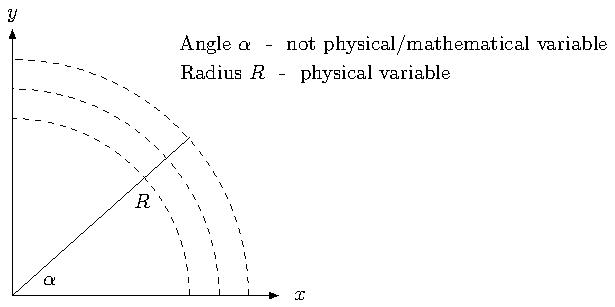
\includegraphics[scale=1.4]{img/rotation.pdf}
\end{center}
\caption{Rotations as gauge transformations.}
\label{fig:3}
\end{figure}
So the quantity 
\begin{align}
R = x^2 + y^2 
\end{align}
will not change under these gauge transformations. To see this, notice that
\begin{align}
\delta R = \varepsilon \left \{ x^2 + y^2 , \phi \right \} = \varepsilon \left \{ x^2 + y^2 , p_x y - p_y x \right \} = \varepsilon (2xy - 2yx) = 0.
\end{align}

With a bit of imagination, one could see this faster. The Lagrangian depends only on the radius $R$, not the angle:
\begin{align}
L = \frac{1}{2} (x \dot{x} + y \dot{y})^2 = \frac{1}{8} \left( \frac{d}{dt} (x^2 + y^2) \right)^2 = \frac{1}{8} \left( \frac{d R^2}{dt} \right)^2 = \frac{1}{8} (2 R \dot{R})^2 = \frac{1}{2} R^2 \dot{R}^2.
\end{align}

\label{sec:finite_gauge_transformations}
How to get from infinitesimal transformations to finite transformations in general? \\

We claim that 
\begin{align}
g(\alpha) = \sum_{n=0}^{\infty} \frac{\alpha^n}{n !} \underbrace{\Large \{ \dots \left \{ \left \{ g_0 , \phi \right \} , \phi \right \} \dots \ , \phi \Large \}}_{n \ \text{times}}
\end{align}
is the general solution.
\begin{proof}
\begin{align}
\frac{d g}{d \alpha} &= \sum_{n=1}^{\infty} \frac{\alpha^{n-1}}{(n-1) !} \underbrace{\Large \{ \dots \left \{ \left \{ g_0 , \phi \right \} , \phi \right \} \dots \ , \phi \Large \}}_{n \ \text{times}} \notag \\
&= \sum_{\bar{n}=0}^{\infty} \frac{\alpha^{\bar{n}}}{\bar{n} !} \underbrace{\Large \{ \dots \left \{ \left \{ g_0 , \phi \right \} , \phi \right \} \dots \ , \phi \Large \}}_{\bar{n} + 1 \ \text{times}} \notag \\
&= \left \{ g , \phi \right \}.
\end{align}
\end{proof}
So, one gets the full transformation out of the constraint $\phi$ by 
\begin{align}\label{eq:11}
g(\alpha) = g_0 + \alpha \left\{ g_0 , \phi \right \} + \frac{\alpha^2}{2} \left \{ \left \{ g_0 , \phi \right \} , \phi \right \} + \dots \ .
\end{align}
With this method we can again derive the same result of the last example:
\begin{itemize}
\item $\left\{ x , \phi \right \} = y$
\item $\left \{ \left\{ x , \phi \right \} , \phi \right \} = \left\{ y , \phi \right \} = - x$
\item $\left \{ \left \{ \left\{ x , \phi \right \} , \phi \right \} , \phi \right \} = \left\{ -x , \phi \right \} = - y$
\item $\left \{ \left \{ \left \{ \left\{ x , \phi \right \} , \phi \right \}, \phi \right \}, \phi \right \} = \left\{ -y , \phi \right \} = x$.
\end{itemize}
So we see that
\begin{align}
x(\alpha) &= \sum_{n=0}^{\infty} \frac{\alpha^n}{n !} \Large \{ \dots \left \{ \left \{ x , \phi \right \} , \phi \right \} \dots \ , \phi \Large \} \notag \\
&= \left( x + \frac{\alpha^2}{2} (-x) + \frac{\alpha^4}{4 !} (x) + \dots \right) + \left( \alpha y + \frac{\alpha^3}{3 !} (-y) + \frac{\alpha^5}{5 !} (y) + \dots \right) \notag \\
&= x \cos \alpha + y \sin \alpha.
\end{align}


\pagebreak

\textbf{General Case} \\

We already know that first-class primary constraints generate gauge transformations, but what about secondary constraints? Will they also be first-class and generate gauge transformations?
Dirac could not show this in general but for all physical situations.

\begin{proof}
Let $\phi_1$ and $\phi_2$ be two constraints.
\begin{figure}[H]
\begin{center}
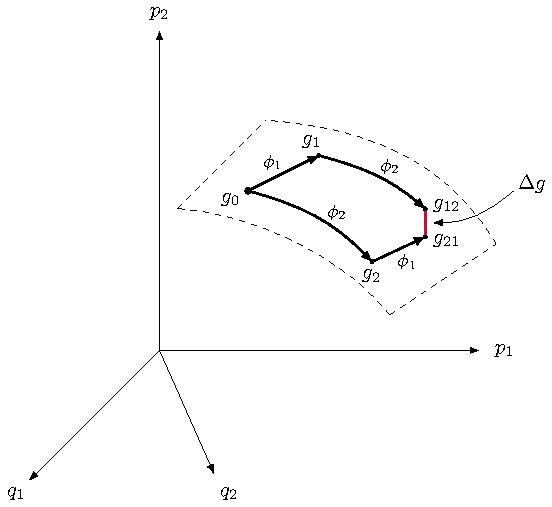
\includegraphics[scale=1.2]{img/gauge2.pdf}
\end{center}
\caption{Different constraints generate different transformations.}
\label{fig:4}
\end{figure}
First, we want to show that transformations between $g_{12}$ and $g_{21}$ are generated by $\left\{ \phi_1 , \phi_2 \right \}$.
We use equation \eqref{eq:11} to the second order to get
\begin{itemize}
\item $g_1 = g_0 + \alpha \left\{ g_0 , \phi_1 \right \} + \frac{\alpha^2}{2} \left \{ \left \{ g_0 , \phi_1 \right \} , \phi_1 \right \} $
\item $g_{12} = g_1 + \beta \left\{ g_1 , \phi_2 \right \} + \frac{\beta^2}{2} \left \{ \left \{ g_1 , \phi_2 \right \} , \phi_2 \right \}  $
\item $g_2 = g_0 + \beta \left\{ g_0 , \phi_2 \right \} + \frac{\beta^2}{2} \left \{ \left \{ g_0 , \phi_2 \right \} , \phi_2 \right \} $
\item $g_{21} = g_2 + \alpha \left\{ g_2 , \phi_1 \right \} + \frac{\alpha^2}{2} \left \{ \left \{ g_2 , \phi_1 \right \} , \phi_1 \right \} .$ 
\end{itemize}
So 
\begin{align}
\Delta g = g_{12} - g_{21} = \dots  = \alpha \beta \left \{ g_0 , \left \{ \phi_1 , \phi_2 \right \} \right \}.
\end{align}
When secondary constraints are first-class then this works out and $\left \{ \phi_1 , \phi_2 \right \}$ is a generator. 

\pagebreak

Now, we want to show that $\left\{ H , \phi_a \right \}$ is also a generator of gauge transformations. 

\begin{figure}[H]
\begin{center}
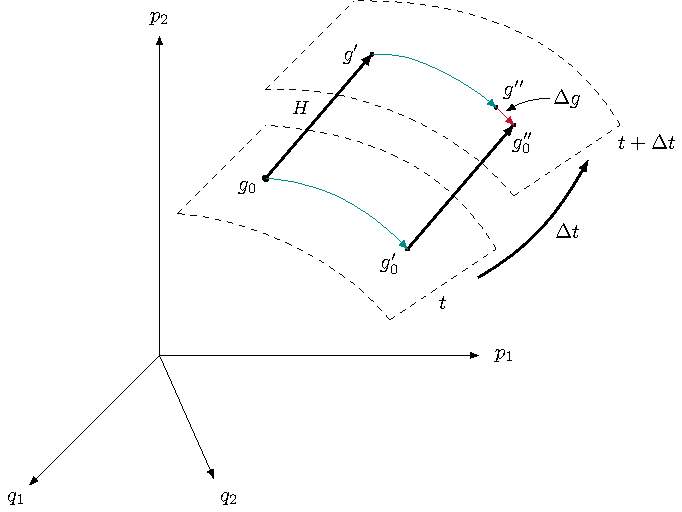
\includegraphics[scale=1.1]{img/gauge3.pdf}
\end{center}
\caption{Physical and mathematical changes of the quantity $g_0$.}
\label{fig:5}
\end{figure}
Consider again
\begin{align}
\frac{\Delta g}{\Delta t} = \left\{ g , H' \right \} + \sum_{a=1}^A v_a \left\{ g , \phi_a \right \}.
\end{align}
We can analyse which part is responsible for which action:
\begin{align}
g' = g(t + \Delta t) = g_0 + \underbrace{\left\{ g_0 , H' \right \} \Delta t}_{\begin{subarray}{l}\text{corresponds to a}\\ \text{physical change}\\
    \text{from layer \ $t \ \rightarrow \ t + \Delta t$.}\end{subarray}}
+ \underbrace{\sum_{a=1}^A \varepsilon_a \left\{ g_0 , \phi_a \right \}}_{\begin{subarray}{2}\text{corresponds to a shift}\\
    \text{within a layer of constant time,}\\
    \text{not physical change.}\end{subarray}}.
\end{align}
Performing a gauge transformation on $g'$ yields:
\begin{align}
g'' = g' + \varepsilon_a \left\{ g' , \phi_a \right \} = g_0 + \left\{ g_0 , H' \right \} \Delta t + 2 \varepsilon_a \left\{ g_0 , \phi_a \right \} + \varepsilon_a \left\{ \left\{ g_0 , H' \right \} \Delta t, \phi_a \right\}.
\end{align}
Now, perform a gauge transformation first
\begin{align}
g_0' = g_0 + \varepsilon_a \left\{ g_0 , \phi_a \right \}
\end{align}
and then calculate the physical change
\begin{align}
g_0'' &= g_0' + \left\{ g_0' , H' \right \} \Delta t + \varepsilon_a \left\{ g_0' , \phi_a \right \} \notag \\
&= g_0 + \left\{ g_0 , H' \right \} \Delta t + 2 \varepsilon_a \left\{ g_0 , \phi_a \right \} + \varepsilon_a \left\{ \left\{ g_0 , \phi_a \right \} , H' \right \} \Delta t.
\end{align}
The difference is 
\begin{align}
\Delta g = g'' - g_0'' &= \varepsilon_a  \left\{ \left\{ g_0 , H' \right \} , \phi_a \right \} \Delta t - \varepsilon_a  \left\{ \left\{ g_0 , \phi_a \right \} , H' \right \} \Delta t \notag \\
&= \varepsilon_a \left\{ g_0 ,  \left\{  H' , \phi_a \right \} \right \} \Delta t ,
\end{align}
which shows that $\left\{  H' , \phi_a \right \}$ is a generator. Both $H'$ and $\phi_a$ are first-class.
\end{proof}

Now that we showed that all first-class quantities generate some kind of gauge transformations, it is reasonable to introduce the following definitions:
\begin{definition}[Total Hamiltonian]
\begin{align}
H_T = H + \sum {\begin{subarray}{l}\text{primary constraints}\\ \text{(first-class)}\end{subarray}}.
\end{align}
\end{definition}

\begin{definition}[Generalized Hamiltonian]
\begin{align}
H_E = H_T + \sum {\begin{subarray}{l}\text{secondary constraints}\\ \text{(first-class)}\end{subarray}}.
\end{align}
\end{definition}

The following example shows a case where all constraints are first-class:
\begin{example}
\begin{align}
L = \frac{1}{2} (\dot{x} - xy)^2
\end{align}
From the definition of the generalized momentum we get the primary constraint
\begin{align}
\phi_1 = p_y = 0
\end{align}
and a secondary constraint from the consistency condition:
\begin{align}
0 = \dot{\phi}_1 \ \ \ \Longrightarrow \ \ \ \phi_2 = p_x = 0.
\end{align}
There are no more constraints. Since both constraints are first-class, we can write the generalized Hamiltonian 
\begin{align}
H_E &= \frac{p_x^2}{2} + xy p_x + v p_y + V p_x \notag \\
&= v p_y + \tilde{V} p_x.
\end{align}
The first constraint $\phi_1 = p_y = 0$ lead to gauge transformations of the form
\begin{align}
\delta y = \varepsilon_1 \left \{ y, p_y \right \} = \varepsilon_1 \\
y \ \longrightarrow \ y' = y + \varepsilon_1
\end{align}
and the second constraint $\phi_2 = p_x = 0$ analogous
\begin{align}
\delta x = \varepsilon_2 \left \{ x, p_x \right \} = \varepsilon_2 \\
x \ \longrightarrow \ x' = x + \varepsilon_2.
\end{align}
\end{example}

\pagebreak

\section{Quantization}

In this section we want to discuss which problems can occur when we try to quantize a Hamiltonian system with constraints.
We will focus on the canonical quantization where we replace every physical observable with an operator and change the Poisson bracket into the commutator:

\begin{align}
q_i \ \longrightarrow \ \hat{q}_i \ \ \ , \ \ \ p_i \ \longrightarrow \ \hat{p}_i.
\end{align}
\begin{align}
\left \{ q_i , p_k \right \} = \delta_{ik} \ \ \longrightarrow \ \ \frac{1}{i \hbar} \left[ \hat{q}_i ,\hat{p}_k \right] = \delta_{ik}.
\end{align}
\begin{align}
\forall g \rightarrow \hat{g} : \ \ \frac{d}{dt} \hat{g} = \frac{1}{i \hbar} \left[ \hat{g} ,\hat{H} \right]  \ \ \Longrightarrow \ \ \hat{H} \psi(q_1, \dots, q_n) = E \psi(q_1, \dots, q_n).
\end{align}

What happens with the constraints? 

They are also replaced by operators and if we act on a wavefunction $\psi$, they will vanish since they vanish on the constraint surface. For first-class constraints this leads to the vanishing of the commutator on the constraint surface:
\begin{align}
\left.
\begin{array}{l}
\hat{\phi}_b \hat{\phi}_a \psi(q_1, \dots, q_n) = 0 \\
\hat{\phi}_a \hat{\phi}_b \psi(q_1, \dots, q_n) = 0
\end{array} \ \right \} \ \
\Longrightarrow \ \ \left[ \hat{\phi}_a ,\hat{\phi}_b \right] \psi = 0.
\end{align}
So for first-class constraints, we can make the transition
\begin{align}
\left \{ \phi_a ,\phi_b \right \} = 0 \ \ \longrightarrow \ \ \left[ \hat{\phi}_a ,\hat{\phi}_b \right] = 0
\end{align}
without problems. 
But if we have second-class constraints, for instance
\begin{align}
\left.
\begin{array}{l}
\chi_1 = q_1 = 0 \\
\chi_2 = p_1 = 0
\end{array} \ \right \} \ \
\Longrightarrow \ \ \left \{ \chi_1 ,\chi_2 \right \} = 1,
\end{align}
it won't work that way and will lead to contradictions:
\begin{align}
\left.
\begin{array}{l}
\hat{p}_1 \hat{q}_1 \psi(q_1, \dots, q_n) = 0 \\
\hat{q}_1 \hat{p}_1 \psi(q_1, \dots, q_n) = 0
\end{array} \ \right \} \ \
\Longrightarrow \ \ \underbrace{\left[ \hat{q}_1 ,\hat{p}_1 \right]}_{= i \hbar} \psi = 0 \ \ \Longrightarrow \ \ \psi = 0.
\end{align}

We can do calculations with the commutator of first-class constraints but not of second-class constraints. 
\begin{align}
H_E = H' + \underbrace{\sum_{a=1}^A v_a \  \tilde{\phi}_a}_{\begin{subarray}{l}\text{primary constraints}\\ \text{(first-class)}\end{subarray}} + \underbrace{\sum v_b \ \tilde{\tilde{\phi}}_b}_{\begin{subarray}{l}\text{secondary constraints}\\ \text{(first-class)}\end{subarray}}.
\end{align}
First-class constraints are generators of gauge transforations and don't change the physical state.
The commutator shows that they are problems with second-class constraints. Let us see how to quantize a Hamiltonian system with second-class constraints. 

\pagebreak

First, we will show that there is always an even number of true second-class constraints (which one cannot combine to first-class constraints). This is good, since every two second-class constraints will lead to a reduction of one degree of freedom.
Mathematically, we will replace the Poisson bracket with the Dirac bracket (which is a generalized Poisson bracket) to fix the problem of second-class constraints.

\label{sec:number_secondary_constraints}
\begin{theorem}
Let $\chi_1, \chi_2, \dots, \chi_S$ be true second-class constraints. Then $S$ is even.
\end{theorem}
%komischer abstand hier ...
\begin{proof}
Introduce the  matrix
\begin{align}
\hat{a}_{ik} = \left \{ \chi_i , \chi_k \right \}, \ \ \ 1 \leq i,k \leq S,
\end{align}
which is obviously antisymmetric because of the antisymmetry of the Poisson bracket. Since the determinant of an odd dimensional antisymmetric matrix is automatically zero, we have to show that $\det (\hat{a}) \neq 0$ which would imply that $S$ is even. \\
Suppose $S$ is odd and $\det (\hat{a}) = 0$. Then $\text{rank}(\hat{a}) = T < S$. \\
Find a minor of $\hat{a}$ which has $\text{rank} = T$ and $\det \neq 0$ and build the \\ $(T+1) \times (T+1)$ - matrix
\begin{align}
\hat{b} =
\left( 
\arraycolsep=1.4pt\def\arraystretch{1.4}
\begin{array}{c|cccc}
\chi_1 & \left\{ \chi_1,\chi_{k_1} \right\} & \left\{ \chi_1,\chi_{k_2} \right\} & \cdots & \left\{ \chi_1,\chi_{k_T} \right\} \\
\chi_2 & \left\{ \chi_2,\chi_{k_1} \right\} & \left\{ \chi_2,\chi_{k_2} \right\} & \cdots & \left\{ \chi_2,\chi_{k_T} \right\} \\
\vdots & \vdots & \vdots & \ddots & \vdots \\
\chi_T & \left\{ \chi_T,\chi_{k_1} \right\} & \left\{ \chi_T,\chi_{k_2} \right\} & \cdots & \left\{ \chi_T,\chi_{k_T} \right\} \\ \cline{1-5}
\chi_{T+1} & \left\{ \chi_{T+1},\chi_{k_1} \right\} & \left\{ \chi_{T+1},\chi_{k_2} \right\} & \cdots & \left\{ \chi_{T+1},\chi_{k_T} \right\} 
\end{array} \right),
\end{align}
where $\chi_{T+1}$ is an arbitrary constraint which is left. We claim that $\det (\hat{b})$ is first-class. This would lead to a contradiction since we can't reach a first-class quantity with true second-class constraints.
Let's show this: \\
\begin{align}
\left\{ \det (\hat{b}),\phi_j \right\} &= 
\det \left( 
\arraycolsep=1.4pt\def\arraystretch{1.4}
\begin{array}{c|cccc}
\left\{ \chi_1,\phi_j \right\} & \left\{ \chi_1,\chi_{k_1} \right\} & \left\{ \chi_1,\chi_{k_2} \right\} & \cdots & \left\{ \chi_1,\chi_{k_T} \right\} \\
\left\{ \chi_2,\phi_j \right\} & \left\{ \chi_2,\chi_{k_1} \right\} & \left\{ \chi_2,\chi_{k_2} \right\} & \cdots & \left\{ \chi_2,\chi_{k_T} \right\} \\
\vdots & \vdots & \vdots & \ddots & \vdots \\
\left\{ \chi_T,\phi_j \right\} & \left\{ \chi_T,\chi_{k_1} \right\} & \left\{ \chi_T,\chi_{k_2} \right\} & \cdots & \left\{ \chi_T,\chi_{k_T} \right\} \\
\left\{ \chi_{T+1},\phi_j \right\} & \left\{ \chi_{T+1},\chi_{k_1} \right\} & \left\{ \chi_{T+1},\chi_{k_2} \right\} & \cdots & \left\{ \chi_{T+1},\chi_{k_T} \right\} 
\end{array} \right) \notag \\[14pt] 
&+ 
\det \left( 
\arraycolsep=1.4pt\def\arraystretch{1.4}
\begin{array}{c|c|ccc}
\chi_1 & \left\{ \left\{ \chi_1,\chi_{k_1} \right\},\phi_j \right\} & \left\{ \chi_1,\chi_{k_2} \right\} & \cdots & \left\{ \chi_1,\chi_{k_T} \right\} \\
\chi_2 & \left\{ \left\{ \chi_2,\chi_{k_1} \right\},\phi_j \right\} & \left\{ \chi_2,\chi_{k_2} \right\} & \cdots & \left\{ \chi_2,\chi_{k_T} \right\} \\
\vdots & \vdots & \vdots & \ddots & \vdots \\
\chi_T & \left\{ \left\{ \chi_T,\chi_{k_1} \right\},\phi_j \right\} & \left\{ \chi_T,\chi_{k_2} \right\} & \cdots & \left\{ \chi_T,\chi_{k_T} \right\} \\
\chi_{T+1} & \left\{ \left\{ \chi_{T+1},\chi_{k_1} \right\},\phi_j \right\} & \left\{ \chi_{T+1},\chi_{k_2} \right\} & \cdots & \left\{ \chi_{T+1},\chi_{k_T} \right\} 
\end{array} \right) \notag \\[14pt] 
&+ \dots \ .
\end{align}
Only the first term is really interesting because we can Laplace expand every other term with respect to the first column and use the fact that $\chi_1, \chi_2, \dots, \chi_{T+1}$ vanish on the constraint surface. \\

Now, there can be several cases: 
\begin{itemize}
\item If $\phi_j$ is first-class, then the Poisson brackets $\left\{ \chi_i,\phi_j \right\}$ will vanish and we are done.
\item If $\phi_j$ is second-class, then it is one of $\chi_1, \dots, \chi_S$ and there are two options:
\begin{enumerate}
\item $\phi_j \in \{ \chi_{k_1}, \dots, \chi_{k_T} \}$, then there will be two equal columns $\Rightarrow \det =0$.
\item $\phi_j \in \{ \chi_{k_{T+1}}, \dots, \chi_{k_S} \}$, then the matrix will be a $(T+1) \times (T+1)$ - minor of the matrix $\hat{a}$ but we fixed $\text{rank} (\hat{a}) = T$, so again $\det = 0$.
\end{enumerate}
\end{itemize}
We showed that $\left\{ \det (\hat{b}),\phi_j \right\} = 0, \ \forall \phi_j$. \\
$\Longrightarrow  \det (\hat{b})$ is a first-class quantity.
\end{proof}

For being able to quantize a Hamiltonian system with second-class constraints, Dirac invented the Dirac bracket:
\label{sec:dirac_bracket}

\begin{definition}[Generalized Dirac bracket]
\begin{align}
\left\{ f,g \right\}_D = \left\{ f,g \right\} - \sum_{i,j = 1}^S \left\{ f,\chi_i \right\} (\hat{a}^{-1})_{ij} \left\{ \chi_j,g \right\}.
\end{align}
\end{definition}

The Dirac bracket has all the properties of the Poisson bracket $+$ fixes the problems:
\begin{enumerate}
\item \(
\begin{aligned}[t]
\left \{ f,g \right \}_D = - \left \{ g,f \right \}_D
\end{aligned} \) \ - \ anticommutative
\item \(
\begin{aligned}[t]
\left \{ \alpha f_1 + \beta f_2,g \right \}_D = \alpha \left \{ f_1,g \right \}_D + \beta \left \{ f_2,g \right \}_D 
\end{aligned} \) \ - \ bilinear
\item \(
\begin{aligned}[t]
\left \{  f_1 f_2,g \right \}_D = f_1 \left \{ f_2,g \right \}_D + f_2 \left \{ f_1,g \right \}_D 
\end{aligned} \) \ - \ "derivative"
\item \(
\begin{aligned}[t]
\left \{ \left \{ f,g \right \}_D,h \right \}_D + \left \{ \left \{ g,h \right \}_D,f \right \}_D + \left \{ \left \{ h,f \right \}_D,g \right \}_D = 0 
\end{aligned} \) \ - \ Jacobi identity
\end{enumerate}

Moreover the equation of motion doesn't change:
\begin{align}
\dot{g} = \left \{ g,H_T \right \}_D = \left \{ g,H_T \right \}
\end{align}
because $H_T$ is a first-class quantity.
The advantage is that every quantity is first-class with the Dirac bracket because the second-class constraints turn to first-class constraints:
\begin{align}
\left \{ g, \chi_j \right \}_D &= \left\{ g,\chi_j \right\} - \sum_{i,k = 1}^S \left\{ g,\chi_i \right\} (\hat{a}^{-1})_{ij} \left\{ \chi_k,\chi_j \right\} \notag \\
&= \left\{ g,\chi_j \right\} - \sum_{i,k = 1}^S \left\{ g,\chi_i \right\} \delta_{ij} \notag \\
&= 0.
\end{align}
In the last section, we said that we have to find all constraints before classifying them. But with the proofed theorem in mind, we don't have to do it anymore since every constraint will be first-class. 

\pagebreak

The following example shows how every two (initially) second-class constraints reduce the degree of freedom by one.

\begin{example}
Consider two second-class constraints:
\begin{align}
\chi_1 &= q_1 = 0 \\
\chi_2 &= p_1 = 0
\end{align}
Then the Dirac bracket is just
\begin{align}
\left \{ f,g \right \}_D &= \left \{ f,g \right \} - \sum_{i,j = 1}^2 \left\{ f,\chi_i \right\} (\hat{a}^{-1})_{ij} \left\{ \chi_j,g \right\} \notag \\
&= \left \{ f,g \right \} - \left\{ f,\chi_1 \right\} (\hat{a}^{-1})_{12} \left\{ \chi_2,g \right\} - \left\{ f,\chi_2 \right\} (\hat{a}^{-1})_{21} \left\{ \chi_1,g \right\} \notag \\
&= \sum_{i=1}^n \left( \frac{\partial f}{\partial q_i} \frac{\partial g}{\partial p_i} - \frac{\partial g}{\partial q_i} \frac{\partial f}{\partial p_i} \right) - \left( - \frac{\partial f}{\partial p_1} \right) (-1) \left( - \frac{\partial g}{\partial q_1} \right) - \left( \frac{\partial f}{\partial q_1} \right) (+1) \left( \frac{\partial g}{\partial p_1} \right) \notag \\
&= \sum_{i=2}^n \left( \frac{\partial f}{\partial q_i} \frac{\partial g}{\partial p_i} - \frac{\partial g}{\partial q_i} \frac{\partial f}{\partial p_i} \right).
\end{align}
\end{example}

Since there is always an even number of true second-class constraints, the Dirac bracket will always reduce to the normal Poisson bracket with fewer degrees of freedom.
\chapter{Field Theory}
\label{sec:field_theory}
In the last sections, we dealt with discrete and finite dimensional problems. Now, we want to extend our theory to an infinite number of degrees of freedom and apply it on field theory. The main difference is that we can analyse not only several points but every point in space at once. Imagine assigning the amplitude $q(\bar{x})$ to each point $\bar{x} \in \mathbb{R}^3$:

\begin{example}  
\begin{align}
L(q_i,\dot{q}_i) = \sum_{i=1}^n \left( \frac{\dot{q}_i^2}{2} - \gamma \frac{q_i^2}{2} \right).
\end{align}
In the finite dimensional case, we just have n oscillating points. 
\begin{align}
L[q_{\bar{x}},\dot{q}_{\bar{x}}] = \int d^3 x \left( \frac{\dot{q}^2(\bar{x})}{2} - \gamma \frac{q^2(\bar{x})}{2} \right).
\end{align}
Now, we have oscillators in every point of space.
\end{example}

In field theory, for instance, we want to know the value of the field $\varphi$ in every point $\bar{x}$, see Fig.~\ref{fig:6}. Of course, there is the option to assign more than one field to every point $\bar{x}$.
One can see that the discrete index $i$ is replaced by the continous variable $\bar{x}$.

\begin{figure}[H]
\begin{center}
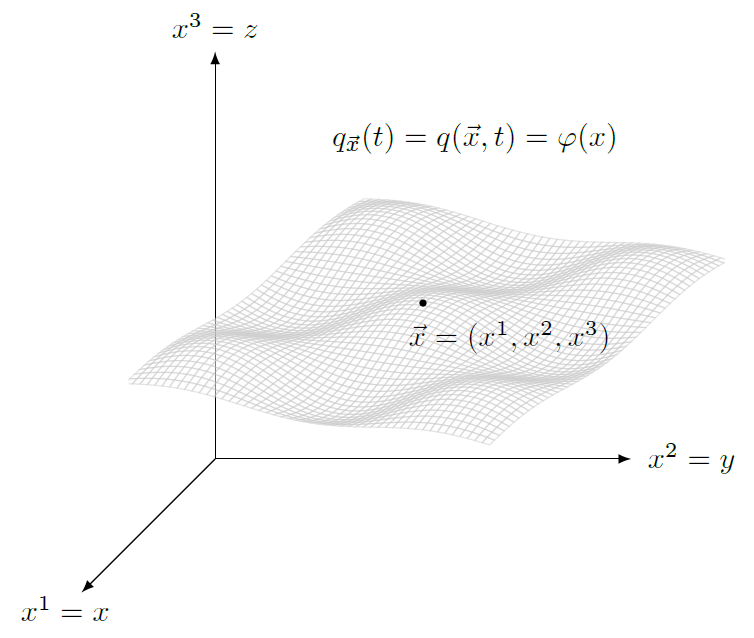
\includegraphics[scale=0.7]{img/field.png}
\end{center}
\caption{Assigning the value of the field $\varphi$ to each point $\bar{x} \in \mathbb{R}^3$.}
\label{fig:6}
\end{figure}

The difference between finite dimensional and infinite dimensional theory is summerized in the following table: 

\begin{table}[H]
\begin{tabular}{>{\centering}p{.45\textwidth} | >{\centering}p{.45\textwidth}} 
Discrete case \vspace{5pt} & Continuous case \vspace{5pt} \tabularnewline \hline 
\vspace{5pt} $q_i(t), \ \ \ i=1, \dots, n$ & \vspace{5pt} $q_{\bar{x}}(t) = q(\bar{x},t), \ \ \ \bar{x} \in \mathbb{R}^3$ \tabularnewline 
\vspace{3pt} $\sum_{i=1}^n$ & \vspace{3pt} $\int d^3 x$ \tabularnewline 
\vspace{3pt} $L(q_1, \dots, q_n, \dot{q}_1, \dots, \dot{q}_n)$ & \vspace{3pt} $L[q_{\bar{x}}, \dot{q}_{\bar{x}}]$ \tabularnewline 
\end{tabular}
\caption{Comparison between finite dimensional and infinite dimensional theory.}
\end{table}

We want our theory to be relativistic invariant, so we have to make our fields dependent on time $q(t, \vec{x}) = q(x^{\mu})$ and build the Lagrangian out of Lorentz scalars:
\begin{align}
L = \frac{1}{2} \int d^3 x \left( \dot{q}^2 - \gamma q^2 \right) \ \ \longrightarrow \ \ \frac{1}{2} \int d^3 x \left( \partial_{\mu} q \partial^{\mu} q - \gamma q^2 \right),
\end{align}
where $\mu = 0,1,2,3$. If we apply a Lorentz transformation on the old Lagrangian, space and time are mixed together so that we get a different result. The new Lagrangian should be build in a way to compensate this mixing and leave the action invariant under Lorentz transformations. We will use the $(+ - - -)$ signature of Minkowski spacetime. \\
The simplest example for such a relativistic invariant field theory is the Klein-Gordon-Fock field:

\begin{example}[Klein-Gordon-Fock field]
\begin{align}
L[\varphi, \dot{\varphi}] &= \frac{1}{2} \int d^3 x \left( \partial_{\mu} \varphi \partial^{\mu} \varphi - m^2 \varphi^2 \right) \notag \\
&= \frac{1}{2} \int d^3 x \left( \dot{\varphi}^2 - (\nabla \varphi)^2 - m^2 \varphi^2 \right) \notag \\
&= \frac{1}{2} \int d^3 x \left( \dot{\varphi}^2 + \varphi \Delta \varphi - m^2 \varphi^2 \right) \notag \\
&= \frac{1}{2} \int d^3 x \left( \dot{\varphi}^2 + \varphi (\Delta - m^2) \varphi \right).
\end{align}
This Lagrangian is regular, so no constraints appear.
\end{example}

We would like to illustrate the Hamiltonian formulation of field theory with the KGF field. The above form of the Lagrangian will be useful later. \\
The next step is to find the Hamiltonian from a given Lagrangian. In the discrete case, we used to differentiate the Lagrangian with respect to the generalized velocities to find the conjugated momenta. What are the generalized velocities now and how to define the conjugated momenta in field theory? To answer this questions, we will need a mathematical tool which we want to develop in the next section. 

\pagebreak

\section{Functional derivative}

The directional derivative for a function $M(q_1, \dots, q_n)$ of $n$ varibles is defined as
\begin{align}
\frac{\partial M}{\partial q_k} = \lim_{a \rightarrow 0} \ \frac{M(q_1, \dots, q_k + a, \dots, q_n) - M(q_1, \dots, q_k, \dots, q_n)}{a}.
\end{align}
We want to generalize the directional derivative for functionals
\begin{align}
M(q_1, \dots, q_n) \ \longrightarrow \ M[q(x)].
\end{align}
The problem is that the functional doesn't depend on the variable $x$ but on the function $q$. For instance, if $x \in [a,b]$, we have to consider every possible path from $a$ to $b$:
\begin{figure}[H]
\begin{center}
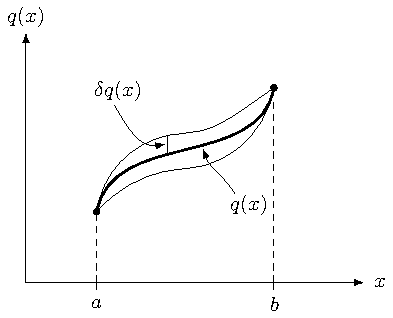
\includegraphics[scale=1.8]{img/variation.pdf}
\end{center}
\caption{Variation of a path $q(x)$ with fixed endpoints.}
\label{fig:7}
\end{figure}
Usually, the knowledge of the complete functional for all possible paths is not required. We rather want to know the behavior of the functional in the vicinity of the function $q$, which makes it extremal or stationary. Therefore, we can take the path $q(x)$ and disturb or variate it by adding a small but arbitrary function $\delta q(x)$. One way of generalizing the directional derivative is by using the variation $\delta M$ of the functional $M[q(x)]$:

\begin{definition}[Functional derivative]
\begin{align}
\delta M \equiv M[q(x) + \delta q(x)] - M[q(x)] = \displaystyle\int\limits_{a}^{b} dx \ \frac{\delta M[q]}{\delta q(x)} \ \delta q(x).
\end{align}
\end{definition}

\pagebreak

If we write $\delta q(x) = \varepsilon \ \eta(x)$, where $\eta(x)$ is an arbitrary function and $\varepsilon$ is infinitesimally small, we can Taylor expand our definition and find:
\begin{align}
\left. \frac{d M[q + \varepsilon \eta]}{d\varepsilon} \ \right|_{\varepsilon=0} = \displaystyle\int\limits_{a}^{b} dx \ \frac{\delta M[q]}{\delta q(x)} \ \eta(x).
\end{align}

This is a useful result to calculate the functional derivative, if one has more complicated functionals. Now, let us look at some simple examples to get comfortable with the definition and understand what's going on.
\vspace{15pt}
\begin{example}
Consider the following functional
\begin{align}
M[q(x)] =  \displaystyle\int\limits_{a}^{b} dx \ q(x).
\end{align}
We can use our definition of the functional derivative
\begin{align}
\delta M = \displaystyle\int\limits_{a}^{b} dx \left( q(x) + \delta q(x) \right) - \displaystyle\int\limits_{a}^{b} dx \ q(x) = \displaystyle\int\limits_{a}^{b} dx \ \delta q(x) \overset{!}{=} \displaystyle\int\limits_{a}^{b} dx \ \frac{\delta M}{\delta q(x)} \ \delta q(x)
\end{align}
and read off the result
\begin{align}
\frac{\delta M}{\delta q(x)} = 1.
\end{align}
\end{example}
\vspace{20pt}
\begin{example}
Next, let us take the functional
\begin{align}
K[q(x)] =  \displaystyle\int\limits_{a}^{b} dx \ q^n(x).
\end{align}
Then, we can use our helpful result
\begin{align}
\left. \frac{d K[q + \varepsilon \eta]}{d\varepsilon} \ \right|_{\varepsilon=0} = \displaystyle\int\limits_{a}^{b} dx \ n q^{n-1}(x) \ \eta(x) \overset{!}{=} \displaystyle\int\limits_{a}^{b} dx \ \frac{\delta K}{\delta q(x)} \ \eta(x) 
\end{align}
to find
\begin{align}
\frac{\delta K}{\delta q(x)} = n q^{n-1}(x).
\end{align}
\end{example}
\vspace{15pt}


One can see that the functional derivative is very similar to the ordinary derivative. In fact, all the properties of the ordinary derivative (like Leibniz rule, chain rule, ...) are satisfied by the functional derivative. We want to show one last useful tool for working with functional derivatives. It is no coincidence that the functional derivative of the above examples looks like the ordinary derivative. \\


More general, we have the property that
\begin{align}
M[q(x)] = \displaystyle\int\limits_{a}^{b} dx \ f(q(x)) \ \ \Longrightarrow \ \ \frac{\delta M}{\delta q(y)} = f'(q(y)).
\end{align}

\begin{proof}
Consider a parametrized family of functionals $M_z[q(x)]$. For a fixed $q$, we can have different outputs depending on $z$. So it looks much like a function with variable $z$:
\begin{align}
M_z[q(x)] \equiv q(z).
\end{align}
By calculating the variation
\begin{align}
\delta M_z &= M_z[q(x) + \delta q(x)] - M_z[q(x)] = q(z) + \delta q(z) - q(z) = \delta q(z) \notag \\
&= \displaystyle\int\limits_{a}^{b} dx \ \delta(x-z) \delta q(x).
\end{align}
we note that 
\begin{align}
\frac{\delta q(z)}{\delta q(x)} \equiv \frac{\delta M_z}{\delta q(x)} = \delta(x-z).
\end{align}
With a bit more work, one can show some more properties of the functional derivative (like changing the order of integration and derivation or the chain rule) and get
\begin{align}
\frac{\delta M}{\delta q(y)} = \displaystyle\int\limits_{a}^{b} dx \ \frac{\delta f(q(x))}{\delta q(y)} = \displaystyle\int\limits_{a}^{b} dx \ f'(q(x)) \frac{\delta q(x)}{\delta q(y)} = f'(q(y)). 
\end{align}
\end{proof}



\section{Hamiltonian description}

Now, we are in the position to continue with the Hamiltonian description of field theory. First, we will define the needed quantities in general and see how the Hamiltonian equations generalizes in field theory. After, we will apply it to the KGF field and see how to interpret the results. Let's go ahead and define the conjugated or generalized momentum for a given field $\varphi$ to be:

\begin{definition}[Generalized momentum]
\begin{align}
\pi(\bar{x}) = \frac{\delta L}{\delta \dot{\varphi}(\bar{x})}.
\end{align}
\end{definition}

The Hamiltonian will be given by
\begin{definition}[Hamiltonian]
\begin{align}
H[\varphi(\bar{x}), \pi(\bar{x})] = \int d^3 x \ \dot{\varphi}(\bar{x}) \pi(\bar{x}) \ - \ L.
\end{align}
\end{definition}


The equation of motion (or time-evolution) is calculated like before
\begin{align}
\dot{g}[\varphi(\bar{x}), \pi(\bar{x})] = \left\{ g,H \right\},
\end{align}
where the Poisson bracket is defined analogous to the discrete case by
\begin{definition}[Poisson bracket]
\begin{align}
\left\{ f,g \right\} \equiv \displaystyle\int d^3 z \left( \frac{\delta f}{\delta \varphi(\bar{z})} \frac{\delta g}{\delta \pi(\bar{z})} - \frac{\delta g}{\delta \varphi(\bar{z})} \frac{\delta f}{\delta \pi(\bar{z})} \right).
\end{align}
\end{definition}

The Hamiltonian equations of motion in field theory take the form:
\begin{align}
\dot{\varphi}(\bar{x}) = \left\{ \varphi(\bar{x}),H \right\} = \displaystyle\int d^3 z \ \frac{\delta \varphi(\bar{x})}{\delta \varphi(\bar{z})} \frac{\delta H}{\delta \pi(\bar{z})} &= \displaystyle\int d^3 z \ \delta^3(\bar{x} - \bar{z}) \frac{\delta H}{\delta \pi(\bar{z})} = \frac{\delta H}{\delta \pi(\bar{x})} \\
\dot{\pi}(\bar{x}) = \left\{ \pi(\bar{x}),H \right\} = - \displaystyle\int d^3 z \frac{\delta H}{\delta \varphi(\bar{z})} \frac{\delta \pi(\bar{x})}{\delta \pi(\bar{z})} &= - \displaystyle\int d^3 z \frac{\delta H}{\delta \varphi(\bar{z})} \delta^3(\bar{x} - \bar{z}) = - \frac{\delta H}{\delta \varphi(\bar{x})}.
\end{align}

Let's apply this results to the Klein-Gordon-Fock field. Remembering the Lagrangian for the KGF field, one gets for the generalized momentum
\begin{align}
\pi(\bar{x}) = \frac{\delta L}{\delta \dot{\varphi}(\bar{x})} = \dot{\varphi}(\bar{x}).
\end{align}
The Hamiltonian can be written as:
\begin{align}
H[\varphi(\bar{x}), \pi(\bar{x})] &= \int d^3 x \ \dot{\varphi}(\bar{x}) \pi(\bar{x}) \ - \ L \notag \\
&= \frac{1}{2} \int d^3 x \left( \pi^2(\bar{x}) + (\nabla \varphi)^2 + m^2 \varphi^2 \right).
\end{align}
The Hamiltonian equations of motion are
\begin{align}
\dot{\varphi}(\bar{x}) &= \frac{\delta H}{\delta \pi(\bar{x})} = \pi(\bar{x}) \label{eq:1h} \\
\dot{\pi}(\bar{x}) &= - \frac{\delta H}{\delta \varphi(\bar{x})} = - m^2 \phi(\bar{x}) - \frac{\delta \left[\displaystyle\int (\nabla \varphi)^2 d^3 y \right]}{2 \ \delta \varphi(\bar{x})} \notag \\
&= - m^2 \phi(\bar{x}) - \displaystyle\int d^3 y \ \nabla \varphi(\bar{y}) \ \frac{\delta (\nabla \varphi(\bar{y}))}{\delta \varphi(\bar{x})} \notag \\
&= - m^2 \phi(\bar{x}) - \displaystyle\int d^3 y \ \nabla_y \varphi(\bar{y}) \ \nabla_y \left( \delta^3(\bar{x}-\bar{y}) \right) \notag \\
&= - m^2 \varphi(\bar{x}) + \displaystyle\int d^3 y \ \Delta \varphi(\bar{y}) \ \delta^3(\bar{x}-\bar{y}) \notag \\
&= - m^2 \varphi(\bar{x}) + \Delta \varphi(\bar{x}). \label{eq:2h}
\end{align}

Differentiating equation \eqref{eq:1h} and inserting equation \eqref{eq:2h} yields
\begin{align}
\ddot{\varphi}(t, \bar{x}) = \dot{\pi}(t, \bar{x}) = (\Delta - m^2) \ \varphi(t, \bar{x}),
\end{align}
which is nothing less than the Klein-Gordon-Fock equation.


\begin{definition}[Klein-Gordon-Fock equation]
\begin{align}
(\partial_{\mu} \partial^{\mu} + m^2) \ \varphi(x^{\nu}) = 0. 
\end{align}
\end{definition}

\vspace{10pt}

Now, we want to analyse this equation a bit further. Its general solution is:
\begin{align}\label{eq:KGF}
\varphi(t,\bar{x}) = \displaystyle\int d^3 k \ c_1(\bar{k}) \ \text{e}^{i k_{\mu} x^{\mu}} + \displaystyle\int d^3 k \ c_2(\bar{k}) \ \text{e}^{- i k_{\mu} x^{\mu}},
\end{align}
where $c_1(\bar{k}), c_2(\bar{k})$ are complex coefficients for each $\bar{k}$. If $c_2(\bar{k}) = c_1^*(\bar{k})$, the field $\varphi(t,\bar{x})$ is real-valued. One can easily derive a condition which $k_{\mu}$ must satisfy in order to be a solution of the KGF equation. Inserting the plane wave exponential into the KGF equation, we get 
\begin{alignat*}{2}
    &\qquad& (\partial_{\mu} \partial^{\mu} + m^2) \text{e}^{i k_{\mu} x^{\mu}} &= 0 \\
    &\Leftrightarrow& \left((i k_0)^2 - (- i \bar{k})^2 + m^2 \right) \text{e}^{i k_{\mu} x^{\mu}} &= 0 \\
    &\Leftrightarrow& \left( - k_0^2 + \bar{k}^2 + m^2 \right) \text{e}^{i k_{\mu} x^{\mu}} &= 0 .
\end{alignat*}
Since the exponential isn't zero, it follows that we must have
\begin{align}
k_0 = \pm \sqrt{m^2 + \bar{k}^2}
\end{align}
for a solution of the KGF equation. This is the relativistic dispersion relation for a particle with
mass $m$. That's why we really can interpret the quadratic terms in the fields like mass terms. From here, it follows also that we have two solutions, one with positive frequency and one with negative frequency. If we change $\bar{k} \rightarrow -\bar{k}$, the sign of the space part does change too but the time part stays the same:
\begin{align}
k_{\mu} x^{\mu} = \sqrt{m^2 + \bar{k}^2} \ t - \bar{k} \bar{x}.
\end{align} 
That's why we can split the general solution into two parts like in \eqref{eq:KGF}. Since the KGF Lagrangian is regular, we have no constraints. In electrodynamics, this is not the case anymore and we will see how constraints enter into the Hamiltonian description.
\chapter{Electrodynamics}
In this chapter, we would like to present an important example of field theory. We want to focus on the Hamiltonian description of electrodynamics and see that it yields the classical results. The Lagrangian of the free electromagnetic field without charges is
\begin{align}
L[A^{\mu}(\bar{x}), \dot{A}^{\mu}(\bar{x})]  = - \frac{1}{4} \displaystyle\int d^3 x \ F_{\mu \nu}(\bar{x}) F^{\mu \nu}(\bar{x}),
\end{align}
where we use natural units and
\begin{align}
F_{\mu \nu}(\bar{x}) = \partial_{\mu} A_{\nu}(\bar{x}) - \partial_{\nu} A_{\mu}(\bar{x})
\end{align}
is the antisymmetric field tensor. Since it is expressed through the vector potential $A^{\mu}(\bar{x})$, the vector potential takes the role of our field $\varphi(\bar{x})$. Note that we have four different fields, since $\mu = 0,1,2,3$.
That's why we define the generalized momenta to be
\begin{align}
\pi_{\rho}(\bar{y}) = \frac{\delta L}{\delta \dot{A}^{\rho}(\bar{y})}.
\end{align}
Inserting the Lagrangian, one gets
\begin{align}
\pi_{\rho}(\bar{y}) &= \frac{\delta L}{\delta \dot{A}^{\rho}(\bar{y})} = - \frac{1}{4} \int d^3 x \ \frac{\delta \left( F_{\mu \nu}(\vec{x}) F^{\mu \nu}(\bar{x}) \right)}{\delta \dot{A}^{\rho}(\bar{y})} \notag \\
&= - \frac{1}{2} \int d^3 x \ F_{\mu \nu}(\bar{x}) \ \frac{\delta \left(\partial^{\mu} A^{\nu}(\bar{x}) - \partial^{\nu} A^{\mu}(\bar{x}) \right)}{\delta \dot{A}^{\rho}(\bar{y})} \notag \\
&= - \frac{1}{2} \int d^3 x \ F_{\mu \nu}(\bar{x}) \left( \delta_0^{\mu} \ \frac{\delta \dot{A}^{\nu}(\bar{x})}{\delta \dot{A}^{\rho}(\bar{y})} - \delta_0^{\nu} \ \frac{\delta \dot{A}^{\mu}(\bar{x})}{\delta \dot{A}^{\rho}(\bar{y})} \right) \notag \\
&= - \frac{1}{2} \int d^3 x \ F_{\mu \nu}(\bar{x}) \left( \delta_0^{\mu} \delta_{\rho}^{\nu} \ \delta^3(\bar{x} - \bar{y}) - \delta_0^{\nu} \delta_{\rho}^{\mu} \ \delta^3(\bar{x} - \bar{y}) \right) \notag \\
&= - \frac{1}{2} \int d^3 x \ \left( F_{0 \rho}(\bar{x}) \ \delta^3(\bar{x} - \bar{y}) - F_{\rho 0}(\bar{x}) \ \delta^3(\bar{x} - \bar{y}) \right) \notag \\
&= - \frac{1}{2} \left( F_{0 \rho}(\bar{y}) - F_{\rho 0}(\bar{y}) \right) = F_{\rho 0}(\bar{y}) .
\end{align}
Using the explicit formula for $F_{\mu \nu}$, the generalized momenta can be written as
\begin{align}
\pi_{\rho}(\bar{y}) = \partial_{\rho} A_0(\bar{y}) - \dot{A}_{\rho}(\bar{y}).
\end{align}
\label{sec:electrodynamics_primary_constraints}
To find the Hamiltonian, one has to invert this equation and express $\dot{A}_{\rho}(\vec{y})$ through $\pi_{\rho}(\vec{y})$ and the field components. We see that this won't be possible for $\rho = 0$, we have a primary constraint:
\begin{align}
\pi_0(\bar{y}) = \partial_0 A_0(\bar{y}) - \dot{A}_0(\bar{y}) = 0 \ \ \ \Longrightarrow \ \ \ \phi_1 = \pi_0(\bar{y}) = 0 \ \ \forall \bar{y} \in \mathbb{R}^3.
\end{align}
More exactly, we have infinitly many constraints because the momentum $\pi_0(\bar{y})$ vanishes in every point in space. This corresponds to the gauge freedom of $A^0(\bar{x})$ as we will see later. No matter how we choose it, the conjugated momentum vanishes identically. For the other components, everything is fine and no more constraints arise. \\
\label{sec:electrodynamics_hamiltonian}
The Hamiltonian is therefore
\begin{align}
H[A^{\mu}(\bar{x}), \pi_{\mu}(\bar{x})] &= \int d^3 x \ \dot{A}^{\mu}(\bar{x}) \pi_{\mu}(\bar{x}) \ - \ L[A^{\mu}(\bar{x}), \dot{A}^{\mu}(\bar{x})] \notag \\
&= \int d^3 x \ \dot{A}^{\mu}(\bar{x}) \pi_{\mu}(\bar{x}) \ + \  \frac{1}{4} \displaystyle\int d^3 x \ F_{\mu \nu}(\bar{x}) F^{\mu \nu}(\bar{x}) \notag \\
&= \int d^3 x \left( \dot{A}^{i}(\bar{x}) \pi_{i}(\bar{x}) + \frac{1}{2} F_{i 0}(\bar{x}) F^{i 0}(\bar{x}) + \frac{1}{4} F_{i k}(\bar{x}) F^{i k}(\bar{x}) \right) \notag \\
&= \int d^3 x \left( \left( \pi_i(\bar{x}) - \partial_i A_0(\bar{x}) \right) \pi_i(\bar{x}) + \frac{1}{2} \pi_i(\bar{x}) (- \pi_i(\bar{x})) + \frac{1}{4} F_{i k}(\bar{x}) F^{i k}(\bar{x}) \right) \notag \\
&= \int d^3 x \left( \frac{1}{2} \pi_i(\bar{x})\pi_i(\bar{x}) - \partial_i A_0(\bar{x}) \pi_i(\bar{x}) + \frac{1}{4} F_{i k}(\bar{x}) F^{i k}(\bar{x}) \right) \notag \\
&= \int d^3 x \left( \frac{1}{2} \pi_i(\bar{x})\pi_i(\bar{x}) + A_0(\bar{x}) \partial_i \pi_i(\bar{x}) + \frac{1}{4} F_{i k}(\bar{x}) F^{i k}(\bar{x}) \right),
\end{align}
where in the last step we integrated by parts and assumed that the fields vanish at infinity. Terms like $\pi_i(\bar{x})\pi_i(\bar{x})$, where both indices are down or up, denote usual summation. \\ 
The first term contains the momenta and is equivalent to the kinetic energy. The last term contains spatial derivatives of the fied components and is therefore equivalent to a potential energy. The second term is a mix of kinetic and potential energy and should not appear in a regular Hamiltonian. We have to check whether the consistency condition for our primary constraint is fulfilled or we have secondary constraints. \\
The total Hamiltonian is 
\begin{align}
H_T = H + \int d^3 x \ u(\bar{x}) \pi_0(\bar{x}).
\end{align}
And the equation of motion is given by 
\begin{align}
\dot{g} = \left \{ g,H_T \right \} = \left \{ g,H \right \} + \int d^3 x \ u(\bar{x}) \left \{ g,\pi_0(\bar{x}) \right \},
\end{align}
where the Poisson bracket is given by
\begin{align}
\left \{ f,g \right \} = \int d^3 z \left( \frac{\delta f}{\delta A^{\mu}(\bar{z})} \frac{\delta g}{\delta \pi_{\mu}(\bar{z})} - \frac{\delta g}{\delta A^{\mu}(\bar{z})} \frac{\delta f}{\delta \pi_{\mu}(\bar{z})}  \right),
\end{align}
analog to the definition in field theory. It follows that
\begin{align}
0 \overset{!}{=} \dot{\pi}_0(\bar{y}) &= \left \{ \pi_0(\bar{y}),H(\bar{y}) \right \} + \int d^3 x \ u(\bar{x}) \left \{ \pi_0(\bar{y}),\pi_0(\bar{x}) \right \} \notag \\
&= - \int d^3 z \ \frac{\delta \pi_0(\bar{y})}{\delta \pi_{\mu}(\bar{z})} \frac{\delta H(\bar{y})}{\delta A^{\mu}(\bar{z})} = - \frac{\delta H(\bar{y})}{\delta A^0(\bar{y})} \notag \\
&= - \int d^3 x \ \partial_i \pi_i(\bar{x}) \frac{\delta A^0(\bar{x})}{\delta A^0(\bar{y})} = - \partial_i \pi_i(\bar{y}).
\end{align}
\label{sec:electrodynamics_secondary_constraints}
So we really get a secondary constraint which is
\begin{align}
\phi_2 = \partial_i \pi_i = \text{div} \ \bar{\pi} = 0.
\end{align}
Again we have to proof that this constraint is fulfilled at every moment (if not, then the primary constraint wouldn't be fulfilled at every moment). \\
It follows that
\begin{align}
0 \overset{!}{=} \frac{d}{dt} \Big( \partial_i \pi_i(\bar{y}) \Big) &= \left \{ \partial_i \pi_i(\bar{y}),H(\bar{y}) \right \} + \int d^3 x \ u(\bar{x}) \left \{ \partial_i \pi_i(\bar{y}),\pi_0(\bar{x}) \right \} \notag \\
&= - \int d^3 z \ \frac{\delta (\partial_i B_i(\bar{y}))}{\delta B_{\mu}(\bar{z})} \frac{\delta H(\bar{y})}{\delta A^{\mu}(\bar{z})} = - \int d^3 z \  \partial_i \left(\delta^3(\bar{y} - \bar{z})\right) \frac{\delta H(\bar{y})}{\delta A^i(\bar{z})} \notag \\
&= - \partial^i \left( \frac{\delta H(\bar{y})}{\delta A^i(\bar{y})} \right),
\end{align}
where the variation is given by 
\begin{align}
\frac{\delta H(\bar{y})}{\delta A^i(\bar{y})} &= \frac{\delta}{\delta A^i(\bar{y})} \left( \frac{1}{4} \int d^3 x \ F_{lk}(\bar{x})F^{lk}(\bar{x}) \right) \notag \\
&= \frac{1}{2} \int d^3 x \ F_{lk}(\bar{x}) \frac{\delta F^{lk}(\bar{x})}{\delta A^i(\bar{y})} \notag \\
&= \frac{1}{2} \int d^3 x \ F_{lk}(\bar{x}) \frac{\delta (\partial^l A^k(\bar{x}) - \partial^k A^l(\bar{x}))}{\delta A^i(\bar{y})} \notag \\
&= \frac{1}{2} \int d^3 x \ F_{lk}(\bar{x}) \left( \delta_i^k  \partial^l \left(\delta^3(\bar{x} - \bar{y})\right) - \delta_i^l  \partial^k \left(\delta^3(\bar{x} - \bar{y})\right) \right) \notag \\
&= \frac{1}{2} \int d^3 x \ \left( - \partial^l F_{li}(\bar{x}) + \partial^k F_{ik}(\bar{x}) \right) \delta^3(\bar{x} - \bar{y}) \notag \\
&= - \partial^k F_{ki}(\bar{y}).
\end{align}
In the end, we get
\begin{align}
\frac{d}{dt} \Big( \partial_i \pi_i(\bar{y}) \Big) = \partial^i \partial^k F_{ki}(\bar{y}),
\end{align}
which is clearly zero since we have a contraction of a symmetric with an antisymmetric tensor. So the secondary constraint is automatically conserved and we get no more constraints. \\

Now, that our procedure is finished, we can classify the constraints and say which is first-class and which is second-class.
Since both constraints depends only on the momentum, they are first-class. So one can write the generalized Hamiltonian as
\begin{align}
H_E = H + \int d^3 x \ v(\bar{x}) \pi_0(\bar{x}) + \int d^3 x \ V(\bar{x}) \partial_i \pi_i(\bar{x}),
\end{align}
where $v(\bar{x})$ and $V(\bar{x})$ are arbitrary functions. \\

\label{sec:electrodynamics_transformations}
Since we have two undetermined functions in our Hamiltonian, this corresponds to two degrees of gauge freedom.
Let's see what transformations $g \longrightarrow g' = g + \delta g$ these first-class constraints do generate. \\
We calculate the small shift $\delta g$ analog to the classical discrete case:
\begin{align}
\delta g = \varepsilon_m \left\{ g,\phi_m \right\} \ \ \ \Longrightarrow \ \ \ \delta g = \int d^3 y \ \varepsilon(\bar{y}) \left\{ g,\phi(\bar{y}) \right\}.
\end{align}
We also have a kind of canonical commutation relation
\begin{align}
\left\{ A^{\mu}(\bar{x}), \pi_{\nu}(\bar{y}) \right\} = \delta_{\nu}^{\mu} \ \delta^3(\bar{x} - \bar{y}),
\end{align}
analog to $\left\{ q_i, p_k \right\} = \delta_{ik}$. Now, we are able to determine the gauge transformations generated by the two constraints. 

\begin{itemize}
\item Choosing $g = A^{\mu}(\bar{x})$, we get for the first constraint:
\begin{align}
\delta A^{\mu}(\bar{x}) &= \int d^3 y \ \varepsilon(\bar{y}) \left\{ A^{\mu}(\bar{x}), \pi_0(\bar{y}) \right\} \notag \\
&= \int d^3 y \ \varepsilon(\bar{y}) \ \delta_0^{\mu} \ \delta^3(\bar{x} - \bar{y}) \notag \\
&= \delta_0^{\mu} \ \varepsilon(\bar{x}).
\end{align}
So the first constraint only generates transformations 
\begin{align}
A_0(\bar{x}) \ \longrightarrow \ A'_0(\bar{x}) = A_0(\bar{x}) + \varepsilon(\bar{x})
\end{align}
and leaves the momentum unchanged since $\left\{ \pi_{\mu}(\bar{x}), \pi_0(\bar{y}) \right\} = 0$.
\item The second constraint leaves the momentum unchanged too because of the same reason. Furthermore it leaves $A_0$ unchanged because the constraint contains only spatial terms and the Poisson bracket vanishes. So we have
\begin{align}
\delta A^k(\bar{x}) &= \int d^3 y \ \tilde{\varepsilon}(\bar{y}) \left\{ A^k(\bar{x}), \partial_i \pi_i(\bar{y}) \right\} \notag \\
&= - \int d^3 y \ \tilde{\varepsilon}(\bar{y}) \ \delta_i^k \ \partial^i \left( \delta^3(\bar{x} - \bar{y}) \right) \notag \\
&= \partial^k \tilde{\varepsilon}(\bar{x}).
\end{align}
So the second constraint generates transformations 
\begin{align}
A^k(\bar{x}) \ \longrightarrow \ A'^k(\bar{x}) = A^k(\bar{x}) + \partial^k \tilde{\varepsilon}(\bar{x}),
\end{align}
or in vector notation
\begin{align}
\bar{A}(\bar{x}) \ \longrightarrow \ \bar{A}'(\bar{x}) = \bar{A}(\bar{x}) + \nabla \tilde{\varepsilon}(\bar{x}).
\end{align}
\end{itemize}

So one can write the generalized Hamiltonian as
\begin{align}
H_E &= \int d^3 x \left( \frac{1}{2} \pi_i(\bar{x})\pi_i(\bar{x}) + (A_0(\bar{x}) + V(\bar{x})) \partial_i \pi_i(\bar{x}) + \frac{1}{4} F_{i k}(\bar{x}) F^{i k}(\bar{x}) + v(\bar{x}) \pi_0(\bar{x}) \right) \notag \\
&= \int d^3 x \left( \frac{1}{2} \pi_i(\bar{x})\pi_i(\bar{x}) + V(\bar{x}) \partial_i \pi_i(\bar{x}) + \frac{1}{4} F_{i k}(\bar{x}) F^{i k}(\bar{x}) + v(\bar{x}) \pi_0(\bar{x}) \right),
\end{align}
because of the gauge freedom of $A_0$, and we see that no mixed terms with momenta and coordinates appear. The Hamiltonian is regular and can be devided in a kinetic and potential energy part. \\

Let's analyse the spatial part of the Hamiltonian and see what it means in terms of the electric field $\bar{E}$ and the magnetic field $\bar{B}$. \\
Remembering that the electromagnetic field tensor in natural units is
\begin{align}
F^{\mu \nu} = 
\left( 
\arraycolsep=1.4pt\def\arraystretch{1.2}
\begin{array}{cccc}
0 & - E^1 & - E^2 & - E^3 \\
E^1 & 0 & - B^3 & B^2 \\
E^2 & B^3 & 0 & - B^1 \\
E^3 & - B^2 & B^1 & 0  
\end{array} \right) \ \ \
\text{and} \ \ \
\bar{B} = \nabla \times \bar{A},
\end{align}
the momentum is nothing more than the electric field:
\begin{align}
\pi^i = F^{i 0} = E^i.
\end{align}
Moreover, if one notices that 
\begin{align}
\bar{B}^2 &= \left( \varepsilon_{ijk} \partial^j A^k \right) \left( \varepsilon_{ilm} \partial^l A^m \right) \notag \\
&= \left( \delta_{jl} \delta_{km} - \delta_{jm} \delta_{kl} \right)  \partial^j A^k \partial^l A^m \notag \\
&= \partial_l A_m(\bar{x}) \partial^l A^m(\bar{x}) - \partial_m A_l(\bar{x}) \partial^l A^m(\bar{x}), 
\end{align}
we can rewrite
\begin{align}
F_{i k}(\bar{x}) F^{i k}(\bar{x}) &= \big( \partial_i A_k(\bar{x}) - \partial_k A_i(\bar{x}) \big) \left( \partial^i A^k(\bar{x}) - \partial^k A^i(\bar{x}) \right) \notag \\
&= 2 \left( \partial_i A_k(\bar{x}) \partial^i A^k(\bar{x}) - \partial_i A_k(\bar{x}) \partial^k A^i(\bar{x}) \right) \notag \\
&= 2 \bar{B}^2.
\end{align}
So the spatial part of the Hamiltonian can be written as
\begin{align}
H_E = \int d^3 x \left( \frac{\bar{E}^2(\bar{x})}{2} + \frac{\bar{B}^2(\bar{x})}{2} \right) + \int d^3 x \ V(\bar{x}) \ \nabla \cdot \bar{E}(\bar{x}),
\end{align}
which is the classical result for the energy of the electromagnetic field. The first term is the kinetic term, the second term is the potential and the third term generates the gauge transformation $\bar{A}' = \bar{A} + \nabla \varepsilon$ that leaves the magnetic field $B$ unchanged.
\chapter{Nambu String}

Now, we want to step over from field theory to string theory. In classical field theory, we got information about our fields in different points of spacetime. Here, we don't have points anymore but one-dimensional objects, called strings. At a given moment, one can move along the string that may change with time. So we need two coordinates, if we want to describe an event on the string. Nevertheless, it is important to keep the theory Lorentz invariant, so we have to work in four-dimensional spacetime. A very practical way is to take the two-dimensional surface and embed it into Minkowski spacetime:
\begin{figure}[H]
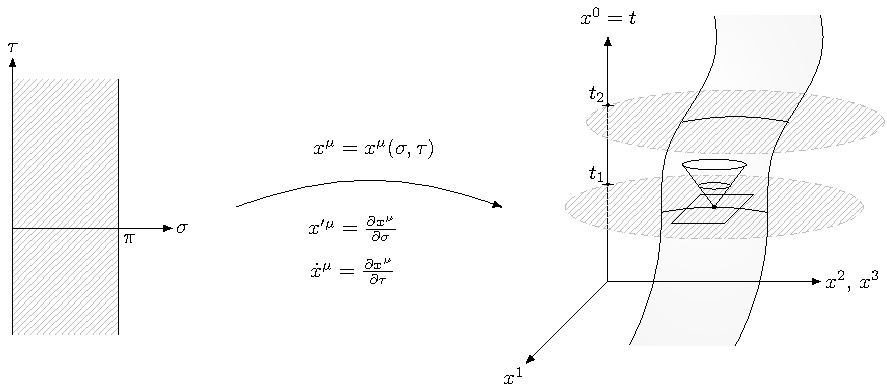
\includegraphics[width=\textwidth]{img/string.pdf}
\caption{Embedding of the Nambu string into Minkowski spacetime}
\label{fig:8}
\end{figure}
Here, $\sigma$ and $\tau$ denote the coordinates of the string at rest (the parametrization) and $x^{\mu}(\sigma, \tau)$ are the coordinates in spacetime. They depend on the inertial observer and can be transformed into each other by a Lorentz transformation. The sections of all embedded points with surfaces of constant time define the string at that moment. We choose $\sigma \in [0,\pi]$ because it is very practical for Fourier transformation which is often used in string theory, but we also could have chosen a different range. \\

Let us see now which conditions the embedding functions $x^{\mu}(\sigma, \tau)$ have to fulfill. First of all, it is very common to consider a closed string, that means identifying the endpoints 
\begin{align}
x^{\mu}(0, \tau) = x^{\mu}(\pi, \tau).
\end{align}
So the worldsheet of the string builds a kind of tube. \\

The second condition is that the string is not allowed to move faster than light ($\bar{v} \leq 1$). If a light signal is emitted on the string, the worldsheet is a cone with apex angle of $90^{\circ}$. The point of emission has to stay in the cone and is not allowed to exit (see Fig.~\ref{fig:8}). This corresponds to
\begin{align}
\dot{x}^2 = (\dot{x}^0)^2 - \dot{\bar{x}}^2 = \left( \frac{dx^0}{d\tau} \right)^2 - \left( \frac{d\bar{x}}{d\tau} \right)^2 \geq 1 - \left( \frac{d\bar{x}}{dx^0} \right)^2 \geq 0.
\end{align}

\pagebreak

And the last condition is that we want to have one time-like and one space-like vector. We found the time-like vector already which is just $\dot{x}^{\mu}$ because of the above condition. So we set the limitation 
\begin{align}
(x')^2 < 0,
\end{align}
and define $x'$ to be the space-like vector. The square should be understand as the inner product with Minkowski metric like in the condition above.


\section{Lagrangian}
What is the Lagrangian for such a string? 
We can try to rewrite the known Lagrangian of a relativistic point particle.
From special relativity, we know that the action of a point particle is 
\begin{align}
S = - m \int \sqrt{1 - \bar{v}^2} \ dt = - m \int \sqrt{(dt)^2 - (d\bar{x})^2} = - m \int \sqrt{dx_{\mu}dx^{\mu}} = - m \int ds. 
\end{align}
We see that the action corresponds to the "length" of the worldline of the particle, measured with Minkowski metric.
\begin{figure}[H]
\begin{center}
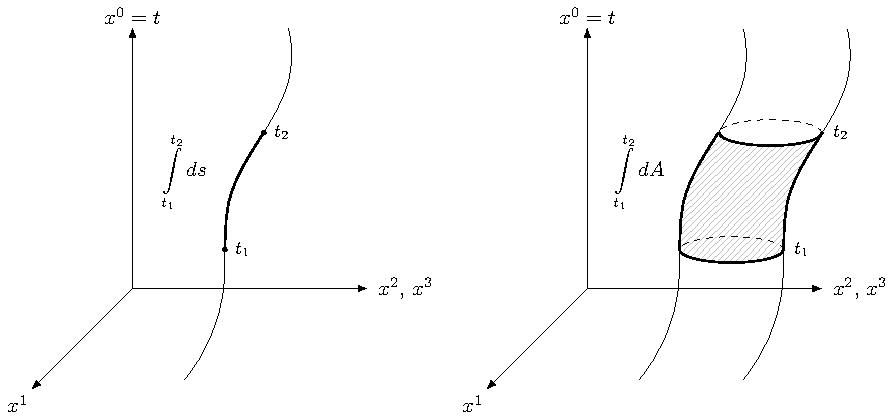
\includegraphics[width=\textwidth]{img/string_action.pdf}
\end{center}
\caption{Action of a relativistic point particle and a relativistic string}
\label{fig:9}
\end{figure}
Since now, we don't have a point which forms a worldline but a string which forms a "worldsuface", it is reasonable to take the area element instead of the line element and define
\begin{align}
S_{\text{str}} \equiv - \gamma \int dA,
\end{align}
where $\gamma$ is a proportionality constant. We will see later that this constant corresponds to the energy per unit length of the string.
But how to find the area element on the worldsheet of the string in Minkowski spacetime? \\

We will need a bit of differential geometry here. The area element on our flat parametrization would be given by $dA = d\sigma d\tau$. When we embed our surface into Minkowski spacetime, we have to consider the changing line elements (see Fig.~\ref{fig:10}):
\begin{align}
da^{\mu} &= \dot{x}^{\mu} d\tau \\
db^{\mu} &= x'^{\mu} d\sigma.
\end{align}
We could take this into account by using the generalized Jacobian determinant but we would like to show a more geometrical way.
\begin{figure}[H]
\begin{center}
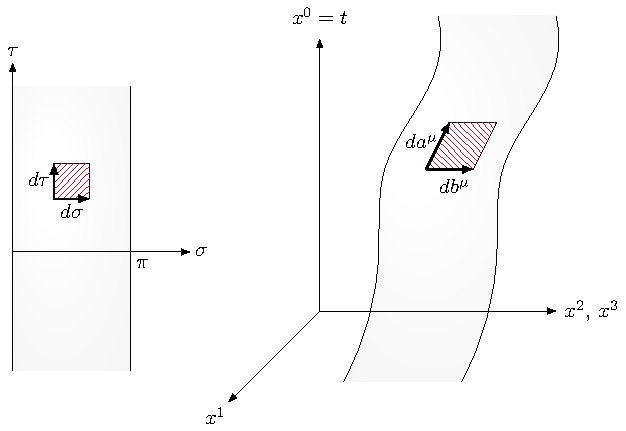
\includegraphics[scale=1.1]{img/string_area.pdf}
\end{center}
\caption{Finding the area element $dA$}
\label{fig:10}
\end{figure}
If an area is spanned by two vectors $\bar{a}, \bar{b}$ in three-dimensional euclidean space, the area is just
\begin{align}
A = |\bar{a} \times \bar{b}| = |\bar{a}| |\bar{b}| \sin(\measuredangle(\bar{a},\bar{b})) = |\bar{a}| |\bar{b}| \sqrt{1 - \left( \frac{\bar{a} \cdot \bar{b}}{|\bar{a}| |\bar{b}|} \right)^2} = \sqrt{|\bar{a}|^2 |\bar{b}|^2 - \left( \bar{a} \cdot \bar{b} \right)^2}.
\end{align}
But how to do it in four-dimensional Minkowski spacetime? If we want to know the area element of an embedded surface, we have to know the induced metric $g_{a b}$ on the surface. In our case, the area element turns out to be very similar to the three-dimensional case
\begin{align}
dA = \sqrt{|g|} \ d\sigma \wedge \tau = \sqrt{(\dot{x}x')^2 - \dot{x}^2(x')^2} \ d\sigma \wedge \tau,
\end{align}
as we will see later. Here $(\dot{x}x')$ denotes the inner product with our Minkowski metric and $x^{\mu}$ still depends on $\sigma$ and $\tau$. So the action for the Nambu string is
\begin{align}
S_{\text{str}} = - \gamma \int dA &= - \gamma \int \sqrt{(\dot{x}x')^2 - \dot{x}^2(x')^2} \ d\sigma d\tau \notag \\
&= - \gamma \displaystyle\int\limits_{\tau_1}^{\tau_2} d\tau \displaystyle\int\limits_{0}^{\pi} d\sigma \sqrt{(\dot{x}x')^2 - \dot{x}^2(x')^2}.
\end{align}


If we identify $\tau$ as the proper time, we can read off the Lagrangian for the Nambu string:
\begin{align}
L[x^{\mu}(\sigma), \dot{x}^{\mu}(\sigma)] = - \gamma \displaystyle\int\limits_{0}^{\pi} d\sigma \sqrt{(\dot{x}x')^2 - \dot{x}^2(x')^2}.
\end{align}




\section{Hamiltonian}

Now that we have the Lagrangian for the Nambu string, we can continue to find the Hamiltonian and see which constraints we get. In some sense, the description of string theory is similar to that of electrodynamics, we just take the coordinates $x^{\mu}$ instead of the fields $A_{\mu}$ and get
\begin{align}
q_i(t) \ \ \longrightarrow \ \ x^{\mu}(\sigma, \tau),
\end{align}
so the index $i$ is now given by $\mu$ and the position $\sigma$ on the string. The generalized momentum is therefore
\begin{align}
p_{\mu}(\sigma) = \frac{\delta L}{\delta \dot{x}^{\mu}(\sigma)}.
\end{align}
Let us calculate it for the Nambu string:
\begin{align}
p_{\mu}(\sigma) &= \frac{\delta L}{\delta \dot{x}^{\mu}(\sigma)} =  - \gamma \displaystyle\int\limits_{0}^{\pi} d\tilde{\sigma} \ \frac{2 (\dot{x}x') \frac{\delta(\dot{x}^{\nu}x'_{\nu})}{\delta \dot{x}^{\mu}(\sigma)} - (x')^2 \frac{\delta (\dot{x}^{\nu}\dot{x}_{\nu})}{\delta \dot{x}^{\mu}(\sigma)}}{2 \sqrt{(\dot{x}x')^2 - \dot{x}^2(x')^2}} \notag \\
&= - \gamma \displaystyle\int\limits_{0}^{\pi} d\tilde{\sigma} \ \frac{(\dot{x}x') \delta_{\mu}^{\nu} \delta(\sigma - \tilde{\sigma}) x'_{\nu} - (x')^2 \dot{x}_{\mu} \delta(\sigma - \tilde{\sigma})}{\sqrt{(\dot{x}x')^2 - \dot{x}^2(x')^2}} \notag \\
&= - \gamma \ \frac{(\dot{x}x') x'_{\mu} - (x')^2 \dot{x}_{\mu}}{\sqrt{(\dot{x}x')^2 - \dot{x}^2(x')^2}},
\end{align}
where the $x^{\mu}$ in the first and second line depend on $\tilde{\sigma}$ and in the last line on $\sigma$. It would be a difficult task to invert this equation and find $\dot{x}_{\mu}(p_{\mu})$ but fortunately we notice that
\begin{align}
px' \equiv p_{\mu}(\sigma) x'^{\mu}(\sigma) = - \gamma \ \frac{(\dot{x}x') (x')^2 - (x')^2 (\dot{x}x')}{\sqrt{(\dot{x}x')^2 - \dot{x}^2(x')^2}} = 0.
\end{align}

Moreover we have
\begin{align}
p^2 \equiv p_{\mu}(\sigma) p^{\mu}(\sigma) &= \gamma^2 \ \frac{(\dot{x}x')^2 (x')^2 - 2 (x')^2 (\dot{x}x')^2 + (x')^4 \dot{x}^2}{(\dot{x}x')^2 - \dot{x}^2(x')^2} \notag \\
&= - \gamma^2 \ \frac{(x')^2 \left[ (\dot{x}x')^2 - (x')^2 \dot{x}^2 \right]}{(\dot{x}x')^2 - \dot{x}^2(x')^2} \notag  \\
&= - \gamma^2 (x')^2.
\end{align}
So we get two primary constraints 
\begin{align}
\phi_1(\sigma) &= p(\sigma) x'(\sigma) = 0 \\
\phi_2(\sigma) &= p^2(\sigma) + \gamma^2 x'^2(\sigma) = 0.
\end{align}

These are already all constraints that we can find because in our case:
\begin{align}
\text{Number of constraints} = 4 - \text{rank} \left( \frac{\delta^2 L}{\delta\dot{x}^{\mu} \delta\dot{x}^{\nu}} \right).
\end{align}
One can show by explicit calculation that the rank of this matrix is two and that we only have two constraints but we won't do it here. \\

The next step is to find the Hamiltonian:
\begin{align}
H[x^{\mu}(\sigma), p^{\mu}(\sigma)] &\equiv \displaystyle\int\limits_{0}^{\pi} d\sigma \ \dot{x}_{\mu}(\sigma)p^{\mu}(\sigma) + \gamma \displaystyle\int\limits_{0}^{\pi} d\sigma \sqrt{(\dot{x}x')^2 - \dot{x}^2(x')^2} \notag \\
&= \displaystyle\int\limits_{0}^{\pi} d\sigma \left( - \gamma \frac{(\dot{x}x')^2 - (x')^2 \dot{x}^2}{\sqrt{(\dot{x}x')^2 - \dot{x}^2(x')^2}} + \gamma \sqrt{(\dot{x}x')^2 - \dot{x}^2(x')^2} \right) \notag \\
&= 0.
\end{align}
We notice that it is zero and in fact, we didn't even had to calculate the Hamiltonian because we know from theorem~\ref{Theorem} that 
\begin{equation}
\text{if} \ \ \ L[x^{\mu}(\sigma), \lambda \dot{x}^{\mu}(\sigma)] = \lambda L[x^{\mu}(\sigma), \dot{x}^{\mu}(\sigma)] \ \ \ \ \Longrightarrow \ \ \ \ H[x^{\mu}(\sigma), p^{\mu}(\sigma)] = 0.
\end{equation}

The total Hamiltonian is therefore
\begin{align}
H_T[x^{\mu}(\sigma), p^{\mu}(\sigma)] = \displaystyle\int\limits_{0}^{\pi} d\sigma \Bigg( u_1(\sigma)\underbrace{(p(\sigma)x'(\sigma))}_{=\phi_1(\sigma)} + u_2(\sigma) \underbrace{(p^2(\sigma) + \gamma^2 x'^2(\sigma))}_{=\phi_2(\sigma)}  \Bigg).
\end{align}

Are these constraints conserved at every moment or do we have secondary constraints? \\
We get the equation of motion by
\begin{align}
\dot{g} = \left \{ g,H_T \right \} = \displaystyle\int\limits_{0}^{\pi} d\sigma \left( u_1(\sigma) \left \{ g,\phi_1(\sigma) \right \}  + u_2(\sigma) \left \{ g,\phi_2(\sigma) \right \} \right),
\end{align}

where
\begin{align}
\left \{ f,g \right \} \equiv \displaystyle\int\limits_{0}^{\pi} d\sigma \left( \frac{\delta f}{\delta x^{\mu}(\sigma)} \frac{\delta g}{\delta p_{\mu}(\sigma)} - \frac{\delta g}{\delta x^{\mu}(\sigma)} \frac{\delta f}{\delta p_{\mu}(\sigma)} \right).
\end{align}


We have to check whether
\begin{align}
0 &\overset{?}{=} \dot{\phi}_1(\tilde{\sigma}) = \displaystyle\int\limits_{0}^{\pi} d\sigma \left( u_1(\sigma) \left \{ \phi_1(\tilde{\sigma}),\phi_1(\sigma) \right \}  + u_2(\sigma) \left \{ \phi_1(\tilde{\sigma}),\phi_2(\sigma) \right \} \right) \\
0 &\overset{?}{=} \dot{\phi}_2(\tilde{\sigma}) = \displaystyle\int\limits_{0}^{\pi} d\sigma \left( u_1(\sigma) \left \{ \phi_2(\tilde{\sigma}),\phi_1(\sigma) \right \}  + u_2(\sigma) \left \{ \phi_2(\tilde{\sigma}),\phi_2(\sigma) \right \} \right).
\end{align}

\pagebreak

Using the identity $\left \{ x^{\mu}(\sigma) , p_{\nu}(\tilde{\sigma}) \right \} = \delta_{\nu}^{\mu} \delta(\sigma - \tilde{\sigma})$ and calculating the poisson brackets accurately, one gets:
\begin{align}
\left \{ \phi_1(\tilde{\sigma}),\phi_1(\sigma) \right \} &=  (\phi_1(\sigma) + \phi_1(\tilde{\sigma})) \frac{\partial}{\partial \sigma}\delta(\sigma - \tilde{\sigma}) \\
\left \{ \phi_2(\tilde{\sigma}),\phi_2(\sigma) \right \} &= (\phi_1(\sigma) + \phi_1(\tilde{\sigma})) \frac{\partial}{\partial \sigma}\delta(\sigma - \tilde{\sigma}) \\
\left \{ \phi_1(\tilde{\sigma}),\phi_2(\sigma) \right \} &= (\phi_2(\sigma) + \phi_2(\tilde{\sigma})) \frac{\partial}{\partial \sigma}\delta(\sigma - \tilde{\sigma}).
\end{align}
So when we insert this in the above equations for $\dot{\phi}_1$ and $\dot{\phi}_2$, we see that they can be expressed by the constraints themself and therefore vanish on the constraint surface. \\
So these two constraints are first-class constraints and we get no secondary constraints, $u_1$ and $u_2$ stay arbitrary. \\


Since we have two arbitrary functions in our Hamiltonian, we have mathematical degrees of freedom or gauge freedom. The constraints are generators of gauge transformations. 

What transformations do they generate?
\begin{align}
\delta g = \varepsilon_m \left\{ g,\phi_m \right\} \ \ \ \Longrightarrow \ \ \ \delta g = \displaystyle\int\limits_{0}^{\pi} d\tilde{\sigma} \ \varepsilon(\tilde{\sigma}) \left\{ g,\phi(\tilde{\sigma}) \right\}.
\end{align}

Let's see which transformations $\phi_1$ generates for the coordinates $x^{\mu}$:
\begin{align}
\delta x^{\mu}(\sigma) &=  \displaystyle\int\limits_{0}^{\pi} d\tilde{\sigma} \ \varepsilon_1(\tilde{\sigma}) \left \{ x^{\mu}(\sigma),(p_{\nu}(\tilde{\sigma}) x'^{\nu}(\tilde{\sigma}) ) \right \} \notag \\
&=  \displaystyle\int\limits_{0}^{\pi} d\tilde{\sigma} \ \varepsilon_1(\tilde{\sigma}) x'^{\nu}(\tilde{\sigma}) \left \{ x^{\mu}(\sigma),p_{\nu}(\tilde{\sigma}) \right \} \notag \\
&= \varepsilon_1(\sigma) x'^{\mu}(\sigma) .
\end{align}
How to interpret this result? One can see that this is just the first order of the Taylor expansion of $x^{\mu}(\sigma + \varepsilon_1(\sigma))$:
\begin{align}
x^{\mu}(\sigma) \ \longrightarrow \ \tilde{x}^{\mu}(\sigma) = x^{\mu}(\sigma) + \varepsilon_1(\sigma) x'^{\mu}(\sigma) = x^{\mu}(\overbrace{\sigma + \varepsilon_1(\sigma)}^{= \tilde{\sigma}}).
\end{align}
So the transformation corresponds to a shift of the variable $\sigma$. That's why we have to impose the conditions
\begin{align}
\varepsilon_1(0) = \varepsilon_1(\pi) = 0,
\end{align}
to not exit the interval $[0,\pi]$:
\begin{align}
\tilde{\sigma}(0) &= 0 \\
\tilde{\sigma}(\pi) &= \pi.
\end{align}

It turns out that this transformation is a map from the string to itself. What changes effectively is the parametrization of the string but not the form of the string itself. \\
It's like we would reparametrize a path. Since we have many possible ways to choose a parametrization, this corresponds to a high degree of freedom. \\

For this moment, we don't want to concentrate on the possible gauge transformations. The other transformations can be found easily, analog to the above procedure. Rather, we want to consider a concrete gauge (a concrete value of the arbitrary functions) and see what dynamics follow from it. 


\section{Dynamics}

Let us choose the gauge:
\begin{align}
u_1(\sigma) &= 0 \\
u_2(\sigma) &= \frac{1}{2 \gamma} 
\end{align}

and calculate the Hamiltonian equations of motion for the coordinates:
\begin{align}\label{eq:78}
\dot{x}^{\mu}(\sigma) &= \left \{ x^{\mu}(\sigma), \frac{1}{2 \gamma} \displaystyle\int\limits_{0}^{\pi} d\tilde{\sigma} \left( p^2(\tilde{\sigma}) + \gamma^2 x'^2(\tilde{\sigma}) \right) \right \} \notag \\
&= \frac{1}{2 \gamma} \displaystyle\int\limits_{0}^{\pi} d\tilde{\sigma} \ 2 p^{\mu}(\tilde{\sigma}) \delta(\sigma - \tilde{\sigma}) \notag \\
&= \frac{p^{\mu}(\sigma)}{\gamma}
\end{align}

and for the momenta:
\begin{align}\label{eq:79}
\dot{p}^{\mu}(\sigma) &= \left \{ p^{\mu}(\sigma), \frac{1}{2 \gamma} \displaystyle\int\limits_{0}^{\pi} d\tilde{\sigma} \left( p^2(\tilde{\sigma}) + \gamma^2 x'^2(\tilde{\sigma}) \right) \right \} \notag \\
&= \frac{1}{2 \gamma} \displaystyle\int\limits_{0}^{\pi} d\tilde{\sigma} \ 2 \gamma^2 x'^{\nu}(\tilde{\sigma}) (- \delta^{\mu}_{\nu}) \frac{\partial}{\partial \tilde{\sigma}}\delta(\sigma - \tilde{\sigma}) \notag \\
&= \gamma x''^{\mu}(\sigma).
\end{align}

Inserting these results into our constraints $\phi_1(\sigma)$ and $\phi_2(\sigma)$, we get the conditions
\begin{align}
\dot{x}^2 + (x')^2 &= 0 \\
\dot{x} x' &= 0,
\end{align}
which means that $x'$ and $\dot{x}$ are orthogonal. That is why we call them \textit{orthonormal gauge}.

Moreover we can take the time-derivative of equation \eqref{eq:78} and insert equation \eqref{eq:79} to get the equation of motion
\begin{equation}\label{eq:eom}
\ddot{x}^{\mu}(\sigma, \tau) - x''^{\mu}(\sigma, \tau) = 0.
\end{equation}

This looks much like the equation $\partial_a \partial^a x^{\mu}(\sigma, \tau) = 0$, where $a = 1,2$ denote the derivative with respect to $\tau$ and $\sigma$, with signature $(+ -)$. That's why we would like to show the connection between $1+1$ gravity and the Nambu string before continuing with the dynamics. 

\begin{example}[$1+1$ Gravity] 
We want to illustrate the connection between the string and $1+1$ gravity, that is, one time-dimension and one space-dimension.
When we embed the string in Minkowski space, it can have curvature. What is the metric? 
The easiest way to find out the components of the metric is to look at the invariant line element  
\begin{align}
dx^{\mu} &= \dot{x}^{\mu} d\tau + x'^{\mu} d\sigma \\
ds^2 &= dx_{\mu}dx^{\mu} = \dot{x}^2 (d\tau)^2 + 2 \dot{x} x' d\tau d\sigma + (x')^2 (d\sigma)^2.
\end{align}
From here we can read off the metric since $ds^2 = g_{ab} \ dx^a dx^b$:
\begin{align}
g_{ab} = 
\begin{pmatrix}
    \dot{x}^2 & \dot{x} x' \\
    \dot{x} x' & (x')^2
  \end{pmatrix}
\end{align}
and with our orthonormal gauge conditions, we get
\begin{align}
g_{ab} = 
\begin{pmatrix}
    \dot{x}^2 & 0 \\
    0 & - \dot{x}^2
  \end{pmatrix}
= \dot{x}^2
\begin{pmatrix}
    1 & 0 \\
    0 & -1
  \end{pmatrix},
\end{align}
which is a conformally flat metric.
So we showed that the "worldsurface" of the string (like every two-dimensional Riemannian manifold) is conformally flat. This means that for every point on this surface, one can find a neighborhood that can be mapped to flat space by a conformal transformation (one that preserves orientation and angles locally). 
The signature is $(+ -)$ like expected.

Let's take a closer look at the action of the string again:
\begin{align}
S = - \gamma \int d\tau d\sigma \sqrt{(\dot{x} x')^2 - \dot{x}^2 (x')^2}.
\end{align}
We notice that the expression under the square root is exactly the negative of the determinant of the metric:
\begin{align}
g \equiv \mbox{det}(g_{ab}) = \dot{x}^2(x')^2 - (\dot{x}x')^2.
\end{align}
So we can write the action of the string as
\begin{align}
S = - \gamma \int d\tau d\sigma \sqrt{- g}
\end{align}
which is a kind of Einstein-Hilbert action for $1+1$ gravity, where $\gamma$ plays the role of a gravity constant. In $3+1$ gravity it takes the form 
\begin{align}
S = \frac{1}{2 \kappa} \int d^4 x \ \sqrt{- g} \ (R + \Lambda).
\end{align}
The string can be easily generalized to higher dimensions.
\end{example}


Let us continue with the dynamics of the Nambu string. We have still enough gauge freedom to set 
\begin{align}
t = x^0(\sigma, \tau) = \tau.
\end{align}
This choice is often used and leads to some simplifications in our dynamics. \\

It implies that
\begin{align}
\arraycolsep=1.4pt\def\arraystretch{1.5}
\begin{array}{ll}
\dot{x}^0 = \frac{\partial x^0}{\partial \tau} = \frac{\partial \tau}{\partial \tau} = 1 \ \ \ & \ \ \ x'^0 = 0 \\
\dot{\bar{x}} = \frac{\partial \bar{x}}{\partial \tau} = \frac{\partial \bar{x}}{\partial t} = \bar{v} \ \ \ & \ \ \ \bar{x}' = \frac{\partial \bar{x}}{\partial \sigma},
\end{array} 
\end{align}
which leads in connection with our constraints to
\begin{align}
\dot{x} x' = - (\dot{\bar{x}} \bar{x}') = 0
\end{align}
and 
\begin{align}
\dot{x}^2 + (x')^2 = (1 - \dot{\bar{x}}^2) - (\bar{x}')^2 = 0.
\end{align}
So we can replace our orthonormal gauge conditions by
\begin{align}
\dot{\bar{x}}^2 + (\bar{x}')^2 &= 1 \\
\dot{\bar{x}} \bar{x}' &= 0
\end{align}
and the equation of motion \eqref{eq:eom} turns to
\begin{align}
\ddot{\bar{x}}(\sigma, \tau) - \bar{x}''(\sigma, \tau) = 0.
\end{align}

So all our constraints and the equation of motion reduced to three dimensions.
Let's see how we can rewrite our Lagrangian:
\begin{align}
L &= - \gamma \displaystyle\int\limits_{0}^{\pi} d\sigma \sqrt{(\dot{x}x')^2 - \dot{x}^2(x')^2} \notag \\
&= - \gamma \displaystyle\int\limits_{0}^{\pi} d\sigma \ \sqrt{0 - (1 - \bar{v}^2) (- (\bar{x}')^2)} \notag \\
&= - \gamma \displaystyle\int\limits_{0}^{\pi} d\sigma \ \left| \bar{x}' \right|  \sqrt{1 - \bar{v}^2}.
\end{align}
It reduces also to three dimensions and looks quite similar to the Lagrangian of a relativistic point particle: $L = - m \sqrt{1 - \bar{v}^2}$. Let us define the length $S$ of the string:
\begin{align}
S = \displaystyle\int\limits_{0}^{\pi} d\sigma \ \left| \bar{x}' \right| = \displaystyle\int\limits_{0}^{S} ds.
\end{align} 

Then we get in analogy to the relativitic point particle:
\begin{align}
dm = \gamma \ ds \ \ \ \Longrightarrow \ \ \ \gamma = \frac{dm}{ds}.
\end{align}

We see that $\gamma$ corresponds to the mass/energy of the string per unit length as mentioned before. 
\chapter{Chromodynamics}

In this last chapter we want to give a quick introduction to chromodynamics or the theory of strong interaction. This is really just a small overview of how the theory is built and how we can apply our Hamilton formalism. 
Let's start with a fundamental observation:

\begin{itemize}
\item \textbf{Electrodynamics:} \\
If we want to seperate an electron and a positron, we have to invest a finite energy.
\item \textbf{Chromodynamics:} \\
If we want to seperate a quark and an antiquark, we would need an infinite amount of energy. The field lines form a tube and get closer and closer the more we seperate the particles. The field energy and the fluctuations raise, so that we create new quarks which bind again before we can seperate the old ones. This process is called "color confinement".
\end{itemize}

So the physical properties of these two interactions are very different but the mathematical description is quite similar, as we will see.
One often starts with the postulation of gauge invariance to introduce the theory of chromodynamics. We want to show a different approach with the same result: a matrix-generalization of electrodynamics. 
In the end, we want to find a Lagrangian again and apply the Hamiltonian method. \\

Let us introduce matrices $\hat{T}^a$, where $a = 1, \dots, n$ with the following properties:
\begin{enumerate}
\item $[ \hat{T}^a , \hat{T}^b ] = t^{abc} \hat{T}^c$ \ with real-valued coefficients $t^{abc}$.
\item $\text{tr}(\hat{T}^a \hat{T}^b) = - 2 \delta^{ab}$.
\item $( \hat{T}^a )^\dag = - \hat{T}^a$.
\end{enumerate} 

For $n=3$, we see that the following $3 \times 3$ matrices satisfy the required properties:
\begin{align}
\hat{T}^1 = 
\begin{pmatrix}
0 & 0 & 0 \\
0 & 0 & - 1 \\
0 & 1 & 0 \\  
\end{pmatrix}, \ \ \
\hat{T}^2 = 
\begin{pmatrix}
0 & 0 & 1 \\
0 & 0 & 0 \\
- 1 & 0 & 0 \\  
\end{pmatrix}, \ \ \
\hat{T}^3 = 
\begin{pmatrix}
0 & - 1 & 0 \\
1 & 0 & 0 \\
0 & 0 & 0 \\  
\end{pmatrix}.
\end{align}

In group theory, this is often referred to the three-dimensional representation of SU(2). \footnote{Note that one can define $i \hat{T}^a \equiv \hat{\tilde{T}}^a$ and get the standard property of hermitian matrices: $( \hat{\tilde{T}}^a )^\dag = - \hat{\tilde{T}}^a$.} \\
 
In nature, we observe the case $n=8$ which corresponds to the group SU(3). It turns out that this group describes strong interaction very well. The number 3 can be referred to the 3 colors of chromodynamics. \\

The following developement of the theory doesn't depend on the number $n$ of matrices. For different $n$, we can get a different description. Just remember that $n=8$ is the case of strong interaction (chromodynamics).

\pagebreak

With the help of our matrices, we generalize the theory of electrodynamics in the following way. Instead of one electromagnetic potential field $A_{\mu}$, we take $n$ different electromagnetic potentials $A_{\mu}^a$:
\begin{align*}
\arraycolsep=10pt\def\arraystretch{1.6}
\begin{array}{ccccc}
 &  & Electrodynamics & & Chromodynamics \\
q_i(t) & \longrightarrow & A_{\mu}(\bar{x},t) & \longrightarrow & A_{\mu}^a(\bar{x},t) \\
i & \longrightarrow & \{ \bar{x},\mu \} & \longrightarrow & \{ \bar{x},a,\mu \}
\end{array}
\end{align*}
and define the "gluon field" $\hat{A}_{\mu}(\bar{x},t)$:
\begin{align}
\hat{A}_{\mu}(\bar{x},t) = \sum_{a=1}^n \ A_{\mu}^a(\bar{x},t) \hat{T}^a.
\end{align}

A simple generalization would be:

\begin{itemize}
\item \textbf{Electrodynamics:} 
\begin{align}
L_{el}[A_{\mu}(\bar{x}), \dot{A}_{\mu}(\bar{x})] = - \frac{1}{4} \displaystyle\int d^3 x \ F_{\mu \nu}(\bar{x}) F^{\mu \nu}(\bar{x}) 
\end{align}
with the electromagnetic field tensor $F_{\mu \nu} = \partial_{\mu} A_{\nu} - \partial_{\nu} A_{\mu}$.
\item \textbf{Chromodynamics:} 
\begin{align}
L_{ch}[A_{\mu}^a(\bar{x}), \dot{A}_{\mu}^a(\bar{x})] = \frac{1}{8} \displaystyle\int d^3 x \ \text{tr}\left(\hat{F}_{\mu \nu}(\bar{x}) \hat{F}^{\mu \nu}(\bar{x}) \right) 
\end{align}
with the "gluon field strength tensor" $\hat{F}_{\mu \nu} = \partial_{\mu} \hat{A}_{\nu} - \partial_{\nu} \hat{A}_{\mu}$.
\end{itemize}

When we write it in the form
\begin{align}
\hat{F}_{\mu \nu}(\bar{x}) = \sum_{a=1}^n F_{\mu \nu}^a(\bar{x}) \hat{T}^a ,
\end{align}
we get for the Lagrangian of chromodynamics:
\begin{align}
L_{ch} = - \frac{1}{4} \displaystyle\int d^3 x \ \sum_{a=1}^n \left( F_{\mu \nu}^a F^{a, \mu \nu} \right) .
\end{align}

But such a simple generalization doesn't lead to chromodynamics. We have to add another term and take
\begin{align}
\hat{F}_{\mu \nu} &= \partial_{\mu} \hat{A}_{\nu} - \partial_{\nu} \hat{A}_{\mu} + g [ \hat{A}_{\mu},\hat{A}_{\nu} ] \\
F_{\mu \nu}^a &= \partial_{\mu} A_{\nu}^a - \partial_{\nu} A_{\mu}^a + g t^{abc} A_{\mu}^b A_{\nu}^c
\end{align}
as the gluon field strength tensor analog to the electromagnetic field tensor. \\
This looks very similar to the curvature tensor of differential geometry. In fact, this extra term conserves the antisymmetry and vanishes in the case of electrodynamics ($n=1$). \\
The equations of motion are non-linear now and the principle of superposition doesn't hold anymore (gluon fields interact with each other).

\pagebreak

The Hamiltonian procedure is the same, just a bit more complicated. We define
\begin{align}
A_{\mu}^a(\bar{x}) \ \ \ \longrightarrow \ \ \ \pi_{\mu}^a(\bar{x}) = \frac{\delta L}{\delta \dot{A}^{a, \mu}(\bar{x})}.
\end{align}
Then we build the Hamiltonian and get again a primary constraint.
It turns out that the primary constraint has the same form like in electrodynamics:
\begin{align}
\phi_1 = \pi_0^a(\bar{x}) = 0.
\end{align}

The secondary constraint reads now:
\begin{align}
\phi_2 = \nabla \cdot \bar{\pi}^a + g t^{abc} \left( \bar{A}^b \bar{\pi}^c \right) = 0.
\end{align}

The procedure ends here and both constraints turn out to be first-class.
The last term can be interpreted like the appearance of a charge in analogy to electrodynamics. If this term isn't zero, then we have interaction between different gluons. \\


Which transformations do they generate? 
\begin{align}
\delta g = \varepsilon_a \{ g,\phi_a \}
\end{align}

We generalize this to arbitrary matrices $\hat{\omega}(\bar{x})$ by letting $\omega^a(\bar{x})$ be arbitrary functions:
\begin{align}
\hat{\omega}(\bar{x}) = \sum_{a=1}^n \ \omega^a(\bar{x}) \hat{T}^a.
\end{align}

After calculating the Poisson bracket with the constraints, we see that the space part changes like
\begin{align}
\hat{\bar{A}} \ \ &\longrightarrow \ \ \hat{\bar{A}}' = e^{- \hat{\omega}} \hat{\bar{A}} e^{\hat{\omega}} + e^{- \hat{\omega}} \nabla e^{\hat{\omega}} \\
\hat{\bar{E}} \ \ &\longrightarrow \ \ \hat{\bar{E}}' = e^{- \hat{\omega}} \hat{\bar{E}} e^{\hat{\omega}} 
\end{align}
and $\hat{\omega}^\dag = - \hat{\omega}$ is antihermite because of the properties of $\hat{T}^a$. \\
This is quite similar to electrodynamics, where we had:
\begin{align}
\bar{A}(\bar{x}) \ \ \longrightarrow \ \ \bar{A}'(\bar{x}) = \bar{A}(\bar{x}) + \nabla \omega(\bar{x}) .
\end{align}

One realizes that the field strength cannot be a physical quantity anymore but 
\begin{align}
\text{tr} ( (\hat{\bar{E}}')^2 ) = \text{tr} ( e^{- \hat{\omega}} \hat{\bar{E}} e^{\hat{\omega}} e^{- \hat{\omega}} \hat{\bar{E}} e^{\hat{\omega}} ) = \text{tr} ( \hat{\bar{E}}^2 ),
\end{align}
because of the gauge invariance. \\

Our small overview ends with this short introduction. It is left to say that the theory turns out to be very complicated. Because of the non-linearity, gluons can interact with each other and create new gluons. Curious readers are advised to get familiar with the Yang-Mills theory.
\newpage
\chapter{Exercises}

Execute the whole generalized Hamiltonian procedure with the following Lagrangians and answer the beneath questions.

\begin{exercise}
\begin{align*}
L = \frac{1}{2} (\dot{x} + x \dot{y})^2 
\end{align*}
Primary constraints as generators of gauge transformations for systems with a finite number of degrees of freedom.
\end{exercise}
\begin{solution}
The generalized momenta are
\begin{align*}
p_x &= \frac{\partial L}{\partial \dot{x}} = (\dot{x} + x \dot{y}) \\
p_y &= \frac{\partial L}{\partial \dot{y}} = x (\dot{x} + x \dot{y}).
\end{align*}
We get the constraint 
\begin{align*}
\phi_1 = x p_x - p_y = 0.
\end{align*}
The Hamiltonian is
\begin{align*}
H = p_x \dot{x} + p_y \dot{y} - \frac{1}{2} (\dot{x} + x \dot{y})^2 = p_x (\dot{x} + x \dot{y}) - \frac{1}{2} (\dot{x} + x \dot{y})^2 = \frac{1}{2} p_x^2.
\end{align*}
The total Hamiltonian at the moment is therefore
\begin{align*}
H_T = \frac{1}{2} p_x^2 + u_1 (x p_x - p_y).
\end{align*}
Is the constraint conserved?
\begin{align*}
0 \overset{?}{=} \dot{\phi}_1 = \left \{ \phi_1,H \right \} + u_1 \left \{ \phi_1,\phi_1 \right \} = \left \{ x p_x - p_y,\frac{1}{2} p_x^2 \right \} = p_x^2.
\end{align*}
So, we get a secondary constraint
\begin{align*}
\phi_2 = p_x = 0.
\end{align*}
Checking the conservation of this constraint, we get
\begin{align*}
\dot{\phi}_2 = \left \{ \phi_2,H_T \right \} = \left \{ p_x,\frac{1}{2} p_x^2 \right \} + u_1 \left \{ p_x,x p_x - p_y \right \} = - u_1 p_x \approx 0.
\end{align*}
Now, everything is consistent and we can classify the constraints. Since
\begin{align*}
\left \{ \phi_1,\phi_2 \right \} = \left \{ x p_x - p_y,p_x \right \} = p_x \approx 0,
\end{align*}
both constraints are first-class. \\
Which transformations do they generate?
\begin{align*}
\Delta x &= \varepsilon \left \{ x,\phi_1 \right \} = \varepsilon \left \{ x,x p_x - p_y \right \} = \varepsilon x \\
\Delta y &= \varepsilon \left \{ y,\phi_1 \right \} = - \varepsilon \\
\Delta p_x &= \varepsilon \left \{ p_x,\phi_1 \right \} = - \varepsilon p_x \\
\Delta p_y &= \varepsilon \left \{ p_y,\phi_1 \right \} = 0
\end{align*}
and 
\begin{align*}
\Delta x &= \varepsilon \left \{ x,\phi_2 \right \} = \varepsilon \left \{ x,p_x \right \} = \varepsilon \\
\Delta y &= \varepsilon \left \{ y,\phi_2 \right \} = 0 \\
\Delta p_x &= \varepsilon \left \{ p_x,\phi_2 \right \} = 0 \\
\Delta p_y &= \varepsilon \left \{ p_y,\phi_2 \right \} = 0.
\end{align*}

The role of primary constraints as generators for gauge transformations can be found in section~\vref{sec:gauge_transformations}.
\end{solution}





\begin{exercise}
\begin{align*}
L = \frac{1}{2} \dot{y}^2 + yx\dot{x}
\end{align*}
Connection between infintely small and finite gauge transformations. 
\end{exercise}
\begin{solution}
The generalized momenta are
\begin{align*}
p_x &= \frac{\partial L}{\partial \dot{x}} = yx \\
p_y &= \frac{\partial L}{\partial \dot{y}} = \dot{y}.
\end{align*}
We get the constraint 
\begin{align*}
\phi_1 = p_x - yx = 0.
\end{align*}
The Hamiltonian is
\begin{align*}
H = p_x \dot{x} + p_y \dot{y} - \frac{1}{2} \dot{y}^2 - yx\dot{x} = \frac{1}{2} p_y^2.
\end{align*}
Therefore
\begin{align*}
H_T = \frac{1}{2} p_y^2 + u_1 (p_x - yx).
\end{align*}
Is the constraint conserved?
\begin{align*}
0 \overset{?}{=} \dot{\phi}_1 = \left \{ \phi_1,H_T \right \} = \left \{ p_x - yx,\frac{1}{2} p_y^2 \right \} = - x p_y.
\end{align*}
We get a secondary constraint
\begin{align*}
\phi_2 = x p_y = 0.
\end{align*}
Checking the conservation of this constraint, we get
\begin{align*}
\dot{\phi}_2 = \left \{ \phi_2,H_T \right \} = \left \{ x p_y,\frac{1}{2} p_y^2 \right \} + u_1 \left \{ x p_y,p_x - yx \right \} = u_1 (p_y + x^2),
\end{align*}
which is a condition on $u_1$, saying that $u_1 = 0$. \\
So everything is consistent now and we can classify the constraints. Since
\begin{align*}
\left \{ \phi_1,\phi_2 \right \} \neq 0
\end{align*}
both constraints are second-class. It turns out that they are true second-class constraints and, in agreement with our theorem, the number is even. \\
Since $u_1$ is determined, we have no degrees of freedom and the constraint does not generate gauge transformations. \\

The connection between infintely small and finite gauge transformations can be found in section~\vref{sec:finite_gauge_transformations}.
\end{solution}





\begin{exercise}
\begin{align*}
L = \frac{1}{2} (\dot{x}y + \dot{y}x)^2
\end{align*}
Constraints as generators of gauge transformations in electrodynamics. 
\end{exercise}
\begin{solution}
The generalized momenta are
\begin{align*}
p_x &= \frac{\partial L}{\partial \dot{x}} = y (\dot{x}y + \dot{y}x) \\
p_y &= \frac{\partial L}{\partial \dot{y}} = x (\dot{x}y + \dot{y}x).
\end{align*}
We get the constraint 
\begin{align*}
\phi_1 = x p_x - y p_y = 0.
\end{align*}
The Hamiltonian is
\begin{align*}
H = p_x \dot{x} + p_y \dot{y} - \frac{1}{2} (\dot{x}y + \dot{y}x)^2 = p_x \left(\dot{x} + \frac{x \dot{y}}{y}\right) - \frac{1}{2} \left(\frac{p_x}{y}\right)^2 = \frac{p_x^2}{2 y^2}.
\end{align*}
The total Hamiltonian at the moment is therefore
\begin{align*}
H_T = \frac{p_x^2}{2 y^2} + u_1 (x p_x - y p_y).
\end{align*}
Is the constraint conserved?
\begin{align*}
\dot{\phi}_1 = \left \{ \phi_1,H_T \right \} = \left \{ x p_x - y p_y,\frac{p_x^2}{2 y^2} \right \} = p_x \frac{p_x}{y^2} + y p_x^2 \frac{(-2)}{2 y^3} = 0.
\end{align*}
So it is conserved identically at any time and we get no secondary constraints. The constraint is first-class and generates the following gauge transformations:
\begin{align*}
\Delta x &= \varepsilon \left \{ x,\phi_1 \right \} = \varepsilon \left \{ x,x p_x - y p_y \right \} = \varepsilon x \\
\Delta y &= \varepsilon \left \{ y,\phi_1 \right \} = - \varepsilon y \\
\Delta p_x &= \varepsilon \left \{ p_x,\phi_1 \right \} = - \varepsilon p_x \\
\Delta p_y &= \varepsilon \left \{ p_y,\phi_1 \right \} = \varepsilon p_y.
\end{align*}

Constraints as generators of gauge transformations in electrodynamics can be found in chapter~\vref{sec:electrodynamics_transformations}.
\end{solution}




\begin{exercise}
\begin{align*}
L = \frac{1}{2} (\dot{x}^2 - x^2) + \frac{1}{2} (\dot{y}^2 - y^2) + \dot{x}\dot{y}
\end{align*}
Show that the primary Poisson bracket is also a generator of gauge transformations. 
\end{exercise}
\begin{solution}
The generalized momenta are
\begin{align*}
p_x &= \frac{\partial L}{\partial \dot{x}} = \dot{x} + \dot{y} \\
p_y &= \frac{\partial L}{\partial \dot{y}} = \dot{y} + \dot{x}.
\end{align*}
We get the constraint 
\begin{align*}
\phi_1 = p_x - p_y = 0.
\end{align*}
The Hamiltonian is
\begin{align*}
H &= p_x \dot{x} + p_y \dot{y} - \frac{1}{2} (\dot{x}^2 - x^2) - \frac{1}{2} (\dot{y}^2 - y^2) - \dot{x}\dot{y} \\
&= p_x (\dot{x} + \dot{y}) - \frac{1}{2} (\dot{x} + \dot{y})^2 + \frac{1}{2} (x^2 + y^2) \\
&= \frac{1}{2} p_x^2 + \frac{1}{2} (x^2 + y^2).
\end{align*}
The total Hamiltonian at the moment is therefore
\begin{align*}
H_T = \frac{1}{2} p_x^2 + \frac{1}{2} (x^2 + y^2) + u_1 (p_x - p_y).
\end{align*}
Is the constraint conserved?
\begin{align*}
0 \overset{?}{=} \dot{\phi}_1 = \left \{ \phi_1,H_T \right \} = \left \{ p_x - p_y,\frac{1}{2} p_x^2 + \frac{1}{2} (x^2 + y^2) \right \} = -x + y.
\end{align*}
We get a secondary constraint
\begin{align*}
\phi_2 = y - x = 0.
\end{align*}
Checking the conservation of this constraint, we get
\begin{align*}
0 \overset{!}{=} \dot{\phi}_2 = \left \{ \phi_2,H_T \right \} = \left \{ y - x,\frac{1}{2} p_x^2 + \frac{1}{2} (x^2 + y^2) \right \} + u_1  \left \{ y - x,p_x - p_y \right \} = - p_x - 2 u_1,
\end{align*}
which leaves us with the condition : $2 u_1 = - p_x$. \\
Since the function $u_1$ is determined, we have no degrees of freedom and no gauge transformations. We can see this also because we have no first-class constraints:
\begin{align*}
\left \{ \phi_1,\phi_2 \right \} = \left \{ p_x - p_y,y - x \right \} = 2 \neq 0.
\end{align*} 

To show that the primary Poisson bracket is also a generator of gauge transformations see section~\vref{sec:gauge_transformations}.
\end{solution}




\begin{exercise}
\begin{align*}
L = \frac{1}{2} (\dot{x} + \dot{y})^2 + \frac{1}{2} (x + y)^2
\end{align*}
Transition to Hamiltonian systems with an infinite number of degrees of freedom. \\
Properties of the functional derivative. 
\end{exercise}
\begin{solution}
The generalized momenta are
\begin{align*}
p_x &= \frac{\partial L}{\partial \dot{x}} = (\dot{x} + \dot{y}) \\
p_y &= \frac{\partial L}{\partial \dot{y}} = (\dot{x} + \dot{y}) .
\end{align*}
We get the constraint 
\begin{align*}
\phi_1 = p_x - p_y = 0.
\end{align*}
The Hamiltonian is
\begin{align*}
H &= p_x \dot{x} + p_y \dot{y} - \frac{1}{2} (\dot{x} + \dot{y})^2 - \frac{1}{2} (x + y)^2 \\
&= p_x (\dot{x} + \dot{y}) - \frac{1}{2} (\dot{x} + \dot{y})^2 - \frac{1}{2} (x + y)^2 \\
&= \frac{1}{2} p_x^2 - \frac{1}{2} (x + y)^2.
\end{align*}
The total Hamiltonian at the moment is therefore
\begin{align*}
H_T = \frac{1}{2} p_x^2 - \frac{1}{2} (x + y)^2 + u_1 (p_x - p_y).
\end{align*}
Is the constraint conserved?
\begin{align*}
0 \overset{?}{=} \dot{\phi}_1 = \left \{ \phi_1,H_T \right \} = \left \{ p_x - p_y,\frac{1}{2} p_x^2 - \frac{1}{2} (x + y)^2 \right \} = 0.
\end{align*}
Yes it is and we get no secondary constraints. \\
The function $u_1$ is still arbitrary and $\phi_1$ generates the following gauge transformations:
\begin{align*}
\Delta x &= \varepsilon \left \{ x,\phi_1 \right \} = \varepsilon \left \{ x,p_x - p_y \right \} = \varepsilon \\
\Delta y &= \varepsilon \left \{ y,\phi_1 \right \} = - \varepsilon \\
\Delta p_x &= \varepsilon \left \{ p_x,\phi_1 \right \} = 0 \\
\Delta p_y &= \varepsilon \left \{ p_y,\phi_1 \right \} = 0.
\end{align*}

The transition to Hamiltonian systems with an infinite number of degrees of freedom and the properties of the functional derivative can be found in chapter~\ref{sec:field_theory}.
\end{solution}





\begin{exercise}
\begin{align*}
L = x \dot{y} - y \dot{x} - x - y
\end{align*}
Mechanical analogy to the scalar Klein-Gordon-Fock field.
\end{exercise}
\begin{solution}
The generalized momenta are
\begin{align*}
p_x &= \frac{\partial L}{\partial \dot{x}} = -y \\
p_y &= \frac{\partial L}{\partial \dot{y}} = x.
\end{align*}
We get two constraints:
\begin{align*}
\phi_1 &= p_x + y = 0 \\
\phi_2 &= p_y - x = 0.
\end{align*}
The Hamiltonian is
\begin{align*}
H &= p_x \dot{x} + p_y \dot{y} - x \dot{y} + y \dot{x} + x + y \\
&= x + y.
\end{align*}
The total Hamiltonian at the moment is therefore
\begin{align*}
H_T = x + y + u_1 (p_x + y) + u_2 (p_y - x).
\end{align*}
Are the constraints conserved?
\begin{align*}
0 &\overset{?}{=} \dot{\phi}_1 = \left \{ \phi_1,H_T \right \} = \left \{ p_x + y,x + y \right \} + u_2 \left \{ p_x + y,p_y - x \right \} = -1 + 2 u_2. \\
0 &\overset{?}{=} \dot{\phi}_2 = \left \{ \phi_2,H_T \right \} = \left \{ p_y - x,x + y \right \} + u_1 \left \{ p_y - x,p_x + y \right \} = -1 - 2 u_1.
\end{align*}
We get no secondary constraints. These are just equations that determine $u_1$ and $u_2$, which is clear since our constraints are second-class:
\begin{align*}
\left \{ \phi_1,\phi_2 \right \} \neq 0.
\end{align*}
Since the constraints are second-class and we have no degrees of freedom left, they do not generate gauge transformations. \\

The mechanical analogy to the scalar Klein-Gordon-Fock field is the standard harmonic oscillator.
\end{solution}





\begin{exercise}
\begin{align*}
L = \frac{1}{2} (\dot{x} - y)^2
\end{align*}
Dirac bracket (generalized Poisson bracket).
\end{exercise}
\begin{solution}
The generalized momenta are
\begin{align*}
p_x &= \frac{\partial L}{\partial \dot{x}} = (\dot{x} - y) \\
p_y &= \frac{\partial L}{\partial \dot{y}} = 0.
\end{align*}
We get the constraint 
\begin{align*}
\phi_1 = p_y = 0.
\end{align*}
The Hamiltonian is
\begin{align*}
H &= p_x \dot{x} + p_y \dot{y} - \frac{1}{2} (\dot{x} - y)^2 = p_x (p_x + y) - \frac{1}{2} p_x^2 = \frac{1}{2} p_x^2 + p_x y.
\end{align*}
The total Hamiltonian at the moment is therefore
\begin{align*}
H_T = \frac{1}{2} p_x^2 + p_x y + u_1 p_y.
\end{align*}
Is the constraint conserved?
\begin{align*}
0 \overset{?}{=} \dot{\phi}_1 = \left \{ \phi_1,H_T \right \} = \left \{ p_y,\frac{1}{2} p_x^2 + p_x y \right \} = - p_x.
\end{align*}
We get a secondary constraint 
\begin{align*}
\phi_2 = p_x = 0.
\end{align*}
Checking the consistency condition, we get
\begin{align*}
\dot{\phi}_2 = \left \{ \phi_2,H_T \right \} = \left \{ p_x,\frac{1}{2} p_x^2 + p_x y \right \} + u_1 \left \{ p_x,p_y \right \} = 0.
\end{align*}
Since 
\begin{align*}
\left \{ \phi_1,\phi_2 \right \} = 0
\end{align*}
both constraints are first-class and generate the following gauge transformations:
\begin{align*}
\Delta x &= \varepsilon \left \{ x,\phi_1 \right \} = \varepsilon \left \{ x,p_y \right \} = 0 \\
\Delta y &= \varepsilon \left \{ y,\phi_1 \right \} = \varepsilon \\
\Delta p_x &= \varepsilon \left \{ p_x,\phi_1 \right \} = 0 \\
\Delta p_y &= \varepsilon \left \{ p_y,\phi_1 \right \} = 0
\end{align*}
and
\begin{align*}
\Delta x &= \varepsilon \left \{ x,\phi_2 \right \} = \varepsilon \left \{ x,p_x \right \} = \varepsilon \\
\Delta y &= \varepsilon \left \{ y,\phi_2 \right \} = 0 \\
\Delta p_x &= \varepsilon \left \{ p_x,\phi_2 \right \} = 0 \\
\Delta p_y &= \varepsilon \left \{ p_y,\phi_2 \right \} = 0.
\end{align*}

The Dirac bracket and its properties can be found in section~\vref{sec:dirac_bracket}.
\end{solution}





\begin{exercise}
\begin{align*}
L = \frac{1}{2} (\dot{x} + \dot{y})^2 - \frac{x^2}{2}
\end{align*}
Show that there only exists an even number of secondary constraints.
\end{exercise}
\begin{solution}
The generalized momenta are
\begin{align*}
p_x &= \frac{\partial L}{\partial \dot{x}} = (\dot{x} + \dot{y}) \\
p_y &= \frac{\partial L}{\partial \dot{y}} = (\dot{x} + \dot{y}).
\end{align*}
We get the constraint 
\begin{align*}
\phi_1 = p_x - p_y = 0.
\end{align*}
The Hamiltonian is
\begin{align*}
H &= p_x \dot{x} + p_y \dot{y} - \frac{1}{2} (\dot{x} + \dot{y})^2 + \frac{x^2}{2} = \frac{1}{2} p_x^2 + \frac{x^2}{2}.
\end{align*}
The total Hamiltonian at the moment is therefore
\begin{align*}
H_T = \frac{1}{2} p_x^2 + \frac{x^2}{2} + u_1 (p_x - p_y).
\end{align*}
Is the constraint conserved?
\begin{align*}
0 \overset{?}{=} \dot{\phi}_1 = \left \{ \phi_1,H_T \right \} = \left \{ p_x - p_y,\frac{1}{2} p_x^2 + \frac{x^2}{2} \right \} = - x.
\end{align*}
We get a secondary constraint 
\begin{align*}
\phi_2 = x = 0.
\end{align*}
Checking the consistency condition, we get
\begin{align*}
0 \overset{!}{=} \dot{\phi}_2 = \left \{ \phi_2,H_T \right \} = \left \{ x,\frac{1}{2} p_x^2 + \frac{x^2}{2} \right \} + u_1 \left \{ x,p_x - p_y \right \} = p_x + u_1.
\end{align*}
This leaves us with the condition $u_1 = - p_x$. We note that 
\begin{align*}
\left \{ \phi_1,\phi_2 \right \} = \left \{ p_x - p_y,x \right \} = - 1 \neq 0
\end{align*}
wich means that both constraints are second-class, so we don't have any degrees of gauge freedom. \\

The proof that there only exists an even number of secondary constraints can be found in section~\vref{sec:number_secondary_constraints}.
\end{solution}





\begin{exercise}
\begin{align*}
L = \frac{1}{2} (\dot{x} - \dot{y})^2 - \frac{1}{2} (x + y)^2
\end{align*}
Conservation of secondary constraints in electrodynamics.
\end{exercise}
\begin{solution}
The generalized momenta are
\begin{align*}
p_x &= \frac{\partial L}{\partial \dot{x}} = (\dot{x} - \dot{y}) \\
p_y &= \frac{\partial L}{\partial \dot{y}} = - (\dot{x} - \dot{y}).
\end{align*}
We get the constraint 
\begin{align*}
\phi_1 = p_x + p_y = 0.
\end{align*}
The Hamiltonian is
\begin{align*}
H &= p_x \dot{x} + p_y \dot{y} - \frac{1}{2} (\dot{x} - \dot{y})^2 + \frac{1}{2} (x + y)^2 = \frac{1}{2} p_x^2 + \frac{1}{2} (x + y)^2.
\end{align*}
The total Hamiltonian at the moment is therefore
\begin{align*}
H_T = \frac{1}{2} p_x^2 + \frac{1}{2} (x + y)^2 + u_1 (p_x + p_y).
\end{align*}
Is the constraint conserved?
\begin{align*}
0 \overset{?}{=} \dot{\phi}_1 = \left \{ \phi_1,H_T \right \} = \left \{ p_x + p_y,\frac{1}{2} p_x^2 + \frac{1}{2} (x + y)^2 \right \} = - 2 (x + y).
\end{align*}
We get a secondary constraint 
\begin{align*}
\phi_2 = x + y = 0.
\end{align*}
Checking the consistency condition, we get
\begin{align*}
0 \overset{!}{=} \dot{\phi}_2 = \left \{ \phi_2,H_T \right \} = \left \{ x + y,\frac{1}{2} p_x^2 + \frac{1}{2} (x + y)^2 \right \} + u_1 \left \{ x + y,p_x + p_y \right \} = p_x + 2 u_1.
\end{align*}
This leaves us with the condition $u_1 = - p_x / 2$. We note that 
\begin{align*}
\left \{ \phi_1,\phi_2 \right \} = \left \{ p_x + p_y,x + y \right \} = - 2 \neq 0
\end{align*}
wich means that both constraints are second-class, so we don't have any degrees of gauge freedom. \\

Secondary constraints in electrodynamics can be found in chapter~\vref{sec:electrodynamics_secondary_constraints}.
\end{solution}




\begin{exercise}
\begin{align*}
L = \frac{1}{2} (\dot{x} + \dot{y})^2 + \dot{x} + \dot{y}
\end{align*}
Secondary constraints in electrodynamics.
\end{exercise}
\begin{solution}
The generalized momenta are
\begin{align*}
p_x &= \frac{\partial L}{\partial \dot{x}} = (\dot{x} + \dot{y}) + 1 \\
p_y &= \frac{\partial L}{\partial \dot{y}} = (\dot{x} + \dot{y}) + 1.
\end{align*}
We get the constraint 
\begin{align*}
\phi_1 = p_x - p_y = 0.
\end{align*}
The Hamiltonian is
\begin{align*}
H &= p_x \dot{x} + p_y \dot{y} - \frac{1}{2} (\dot{x} + \dot{y})^2 - \dot{x} - \dot{y} \\
&= p_x (p_x - 1) - \frac{1}{2} (p_x - 1)^2 - p_x + 1 \\
&= \frac{1}{2} p_x^2 - p_x + \frac{1}{2} \\
&= \frac{1}{2} (p_x - 1)^2.
\end{align*}
The total Hamiltonian is therefore
\begin{align*}
H_T = \frac{1}{2} (p_x - 1)^2 + u_1 (p_x - p_y).
\end{align*}
Is the constraint conserved?
\begin{align*}
\dot{\phi}_1 = \left \{ \phi_1,H_T \right \} = \left \{ p_x - p_y,\frac{1}{2} (p_x - 1)^2 \right \} = 0.
\end{align*}
Yes it is, so we get no secondary constraints. The function $u_1$ is still arbitrary and $\phi_1$ generates the following gauge transformations:
\begin{align*}
\Delta x &= \varepsilon \left \{ x,\phi_1 \right \} = \varepsilon \left \{ x,p_x - p_y \right \} = \varepsilon \\
\Delta y &= \varepsilon \left \{ y,\phi_1 \right \} = - \varepsilon \\
\Delta p_x &= \varepsilon \left \{ p_x,\phi_1 \right \} = 0 \\
\Delta p_y &= \varepsilon \left \{ p_y,\phi_1 \right \} = 0.
\end{align*}

Secondary constraints in electrodynamics can be found in chapter~\vref{sec:electrodynamics_secondary_constraints}.
\end{solution}




\begin{exercise}
\begin{align*}
L = \frac{1}{2} (\dot{x} + \dot{y})^2 + \dot{x} + 2 \dot{y}
\end{align*}
Hamiltonian of electrodynamics.
\end{exercise}
\begin{solution}
The generalized momenta are
\begin{align*}
p_x &= \frac{\partial L}{\partial \dot{x}} = (\dot{x} + \dot{y}) + 1 \\
p_y &= \frac{\partial L}{\partial \dot{y}} = (\dot{x} + \dot{y}) + 2.
\end{align*}
We get the constraint 
\begin{align*}
\phi_1 = p_x - p_y + 1 = 0.
\end{align*}
The Hamiltonian is
\begin{align*}
H &= p_x \dot{x} + p_y \dot{y} - \frac{1}{2} (\dot{x} + \dot{y})^2 - \dot{x} - 2 \dot{y} \\
&= p_x \dot{x} + (p_x + 1) \dot{y} - \frac{1}{2} (\dot{x} + \dot{y})^2 - \dot{x} - 2 \dot{y} \\
&= p_x (p_x - 1) - \frac{1}{2} (p_x - 1)^2 - (p_x - 1) \\
&= \frac{1}{2} (p_x - 1)^2.
\end{align*}
The total Hamiltonian is therefore
\begin{align*}
H_T = \frac{1}{2} (p_x - 1)^2 + u_1 (p_x - p_y + 1).
\end{align*}
Is the constraint conserved?
\begin{align*}
\dot{\phi}_1 = \left \{ \phi_1,H_T \right \} = \left \{ p_x - p_y + 1,\frac{1}{2} (p_x - 1)^2 \right \} = 0.
\end{align*}
Yes it is, so we get no secondary constraints. The function $u_1$ is still arbitrary and $\phi_1$ generates the following gauge transformations:
\begin{align*}
\Delta x &= \varepsilon \left \{ x,\phi_1 \right \} = \varepsilon \left \{ x,p_x - p_y + 1 \right \} = \varepsilon \\
\Delta y &= \varepsilon \left \{ y,\phi_1 \right \} = - \varepsilon \\
\Delta p_x &= \varepsilon \left \{ p_x,\phi_1 \right \} = 0 \\
\Delta p_y &= \varepsilon \left \{ p_y,\phi_1 \right \} = 0.
\end{align*}

The Hamiltonian of electrodynamics can be found in chapter~\vref{sec:electrodynamics_hamiltonian}.
\end{solution}




\begin{exercise}
\begin{align*}
L = \frac{1}{2} (\dot{x} - \dot{y})^2 - \dot{x} - \frac{x^2}{2}
\end{align*}
Primary constraints in electrodynamics.
\end{exercise}
\begin{solution}
The generalized momenta are
\begin{align*}
p_x &= \frac{\partial L}{\partial \dot{x}} = (\dot{x} - \dot{y}) - 1 \\
p_y &= \frac{\partial L}{\partial \dot{y}} = -(\dot{x} - \dot{y}).
\end{align*}
We get the constraint 
\begin{align*}
\phi_1 = p_x + p_y + 1 = 0.
\end{align*}
The Hamiltonian is
\begin{align*}
H &= p_x \dot{x} + p_y \dot{y} - \frac{1}{2} (\dot{x} - \dot{y})^2 + \dot{x} + \frac{x^2}{2} \\
&= (-p_y - 1) \dot{x} + p_y \dot{y} - \frac{1}{2} p_y^2 + \dot{x} + \frac{x^2}{2} \\
&= p_y (\dot{y} - \dot{x}) - \frac{1}{2} p_y^2 + \frac{x^2}{2} \\
&= \frac{1}{2} p_y^2 + \frac{x^2}{2}.
\end{align*}
The total Hamiltonian is therefore
\begin{align*}
H_T = \frac{1}{2} p_y^2 + \frac{x^2}{2} + u_1 (p_x + p_y + 1).
\end{align*}
Is the constraint conserved?
\begin{align*}
0 \overset{?}{=} \dot{\phi}_1 = \left \{ \phi_1,H_T \right \} = \left \{ p_x + p_y + 1, \frac{1}{2} p_y^2 + \frac{x^2}{2} \right \} = - x.
\end{align*}
We get a secondary constraint 
\begin{align*}
\phi_2 = x = 0.
\end{align*}
Checking the consistency condition, we get
\begin{align*}
0 \overset{!}{=} \dot{\phi}_2 = \left \{ \phi_2,H_T \right \} = \left \{ x,\frac{1}{2} p_y^2 + \frac{x^2}{2} \right \} + u_1 \left \{ x,p_x + p_y + 1 \right \} = u_1.
\end{align*}
This leaves us with the condition $u_1 = 0$. We note that 
\begin{align*}
\left \{ \phi_1,\phi_2 \right \} = \left \{ p_x + p_y + 1,x \right \} = - 1 \neq 0,
\end{align*}
wich means that both constraints are second-class, so we don't have any degrees of gauge freedom. \\

The primary constraints of electrodynamics can be found in chapter~\vref{sec:electrodynamics_primary_constraints}.
\end{solution}

\end{document}